
\chapter{Statistical Analysis and Results}
\label{chap:statistical}

%\newpage

\section{Introduction}
The set of categorised diphoton candidates are subjected to a statistical interpretation to measure the Higgs boson signal in data and to determine how its properties compare to SM expectations.
This procedure consists of a statistical model that is fitted simultaneously to the \mgg distribution in data for each tag category. 
Separate models are constructed and then combined for signal and background that take into account the contribution of different categories, production modes and systematic uncertainties.

This chapter begins by describing the construction of these models and the inclusion of the associated systematic uncertainties (following \cite{HIG-16-040}). 
After this, the final fit of the model and the statistical interpretation of the result is described with emphasis on how the two different VBF tagging approaches affect the result. 


\section{Statistical Models}
\subsection{Signal Modelling}
The signal modelling aims to construct a signal shape for each category using simulated data samples of the different Higgs production modes.
This is achieved by constructing many parameterised signal shapes: one for each choice of production mode, category and whether the vertex has been correctly identified. 

Furthermore, the Higgs boson mass \mH is not assumed to have a specific value. A parameterisation of the signal shape in terms of \mH is derived from a collection of samples with different \mH.
This is constructed by performing a simultaneous fit over all of the mass points where the parameters of the signal shape are all polynomials of \mH. 
The floating parameters of this fit are then the coefficients of the polynomial. 
This approach is used instead of interpolating the parameters as it leads to fewer parameters per fit and guarantees consistency across mass points. 

This procedure is also used to determine relative normalisation of the RV and WV scenario shapes when they are combined. 
This is given by the vertex selection efficiency derived from simulated data. 
The value is then treated the same way as the other shape parameters in the simultaneous mass point fit. 

Once constructed the different signal shapes from production modes are combined together to produce the signal model for each category. 
The production mode shapes are normalised to their expected signal yield and then summed.



\subsection{Background Modelling}
The background modelling aims to construct a smoothly falling background distribution that takes uncertainty about the choice of functional form into account. This is achieved with a data-driven approach based on the discrete profiling method \cite{env_method}. This technique allows for the estimation of this systematic and its propagation to the final fits as a discrete nuisance parameter without assumptions about underlying processes or functional forms. 

The candidate functions are expressed as a set of function families, each of these are expressed as a sequence where we pick a lowest and highest order form to consider. The maximum order is found via an F-test and the minimum order is found by requiring a minimal level of goodness-of-fit. 
The families considered are polynomials in the Bernstein basis, Laurent series, sums of exponentials, and sums of power laws. 

The functions are fitted to the \mgg sideband data using twice negative likelihood (2NLL) minimisation with an additional regularisation term $n_p$ (number of parameters) to penalise function complexity. 



\section{Systematic Uncertainties}
Systematic uncertainties are propagated to the final fits by including nuisance parameters primarily in the signal model. 
The desription here is taken from the work in \cite{HIG-16-040} unless stated otherwise. 

Systematic error in the signal model is handled in one of three main ways via nuisance parameters that have different effects on the \mgg distribution:
\begin{itemize}[noitemsep]
    \item Shape uncertainties are propagated via nuisance parameters that alter the shape of the Gaussian signal peak position, width and normalisation.
    \item Yield uncertainties are handled by nuisance parameters that scale the \mgg distribution and are subject to a log-normal constraint during the final fit.
    \item Categorisation uncertainties are implemented as category migration nuisance parameters which behave in a similar way to yield uncertainties but will reduce the yield in other categories simultaneously as the category of interest is increased.
\end{itemize}
There is an exception to this scheme with the vertex uncertainty. Here there is a nuisance parameter that controls the relative fraction of the RV/WV signal distributions rather than affecting the shape parameters directly. 

An extra systematic uncertainty from choice of background functional form is propagated to the final fits via the background model as a discrete nuisance parameter. 



\subsection{Theoretical Uncertainties}
Uncertainties from QCD theory calculations have their effects modelled in two ways: uncertainty on the overall yield for a process and uncertainty associated with analysis category migration. 
The migration uncertainties are extracted separately by scaling such that the overall yield is unchanged.  
\begin{itemize}[noitemsep]
    \item {\textbf{QCD scale uncertainty}: yield uncertainty is parameterised separately for renormalisation scale and factorisation scale. 
                                            Category migrations associated with varying these parameters independently and together are also included.}
    \item{\textbf{PDF uncertainties}: There is an uncertainty associated with variation in the signal yield of each production process, and category migration uncertainties.   
        The yield uncertainty is calculated using the procedure from PDF4LHC \cite{PDF4LHC} and the migration uncertainties are computed from the NNPDF3.0 PDF set \cite{NNPDF3} and the MC2Hessian \cite{MC2Hessian} procedure.}
    \item{\textbf{Strong force coupling ($\alpha_{s}$) uncertainty}: evaluated with the same procedure as the PDF uncertainties.}
    \item{\textbf{Underlying event and parton shower uncertainty}: evaluated using simulated data where the modelling of the underlying event and the parton showers have been varied. This manifests primarily as variation in the jets of the analysis and is modelled as a category migration uncertainty. The probability that events move within the categories of the BDT-based VBF tag, or from this tag to Untagged are found to be 7 and 9\%. This was re-evaluated for the DCNN-based VBF tag and found to be unchanged.}
    \item{\textbf{Gluon fusion contamination in \ttH tag categories}: when the Higgs boson is produced by ggH it can be produced in association with a number of jets. As the number of jets becomes large the accuracy of theoretical predictions becomes worse and introduces a systematic uncertainty in ggH contamination of the jet-based tag categories. This manifests in the \ttH tags in multiple ways:
        \begin{itemize}[noitemsep]
            \item[\textbullet] \textbf{Uncertainty due to limited ggH sample size}: only a small quantity of simulated ggH events are accepted into the \ttH tag. This introduces a significant statistical uncertainty on the ggH yield and contributes a 10\% uncertainty.
            \item[\textbullet] \textbf{Uncertainty due to modelling parton showers}: this is estimated by comparing simulation and data for events whose production is dominated by gluon-fusion-type diagrams ($\mathrm{t}\bar{\mathrm{t}}+\mathrm{jets}$ with semi-leptonic $\mathrm{t}\bar{\mathrm{t}}$ decays) binned by the number of jets. The largest discrepancy is in $N_{\mathrm{jets}}\geq{5}$ which corresponds to an uncertainty of 35\%.
            \item[\textbullet] \textbf{Uncertainty due to modelling gluon splitting}: estimated by calculating the difference in the ratio $\sigma(\mathrm{t\bar{t}b\bar{b}})/\sigma(\mathrm{t\bar{t}jj})$ for simulation and data. The fraction of events in simulated ggH with b jets are then scaled by this difference. This gives a 50\% variation in the ggH yield for the \ttH tags. 
        \end{itemize}}
    \item{\textbf{Gluon fusion contamination in tag categories with jets and a high-\pt Higgs boson}: how ggH mismodelling manifests in the VBF categories, in particular:
        \begin{itemize}[noitemsep]
            \item[\textbullet] \textbf{Uncertainty due to jet multiplicity mismodelling}: two nuisance parameters due to missing higher-order terms and two more nuisance parameters for category migration due to variation in jet multiplicity based on STWZ \cite{JetPtResum} and BLPTW \cite{JetPtResum,TheoryUncertHiggs1J,ResummedHiggsPredictions} predictions. 
            \item[\textbullet] \textbf{Uncertainty due to Higgs boson \pt mismodelling}: two nuisance parameters associated with migration between two bins in Higgs boson \pt; from 60 to 120 \,GeV and above 120\,GeV. There is also a third nuisance due to uncertainty in top quark mass effects. This is negligible for \pt less than 150\,GeV but increases to 35\% at 500\,GeV. These impact the highest-score VBF and Untagged categories where the ggH yield uncertainty is 6-8\%.
            \item[\textbullet] \textbf{Uncertainty in the acceptance of ggH in VBF categories due to QCD effects}: effects from missing higher-order terms are estimated via variations in the renormalisation and factorisation scales in MCFM 5.8 \cite{MCFM}. Two nuisance parameters are introduced associated with the overall normalisation of Higgs bosons produced in association with two jets, and three or more jets. This allows for the impact of jet suppression arising from how the kinematic variables are used to form the VBF scores to be propagated to the analysis. The procedure is based on the Stewart-Tackmann method \cite{StewartTackmann,GangalTackmann} and the impact on the ggH yield in the VBF categories is 8-13\%. 
        \end{itemize}}
    \item{\textbf{Uncertainty in the \Hgg branching fraction}: the uncertainty on the theoretical prediction of the \Hgg branching fraction is taken from \cite{LHCHXS} and is approximately 2\%.}
\end{itemize}

The theory uncertainties with the largest impact on measuring signal strengths and couplings are the \Hgg branching fraction, and the renormalisation and factorisation scale uncertainties from the QCD scale. 



\subsection{Experimental Uncertainties}
Uncertainty in the measurement and construction of physics objects at CMS give rises to associated experimental systematic uncertainties. 
These affect the shape of the signal distribution and are propagated through to the final fits via the signal model. 
\subsubsection{Photon Energy Measurement Uncertainties}
Uncertainties in the photon energy measurement are a particularly important contribution and can affect the signal shape via both the photon energy scale and resolution.
\begin{itemize}[noitemsep]
    \item {\textbf{Energy scale and resolution}: 
           uncertainties associated with the photon energy scale and resolution corrections
           are estimated with events from the \Zee control region reconstructed as photons. Data and simulation are compared in eight bins of $R_9$ and $|\eta|$ (high/low-$R_9$, and four $|\eta|$ bins). 
           The uncertainties are quantified separately in four photon classes (EB/EE and high/low-$R_9$) and are propagated to the categorisation with four scale nuisance parameters (one per photon class) and eight shape nuisance parameters (one constant and one stochastic term per photon class) for each event category. 
           This has a 0.15-0.5\% effect on the photon energy, and an effect of 2.5\% on the signal strength modifier. 
           }
    \item {\textbf{Nonlinearity of photon energy}: 
          There is potential residual data-simulation difference in the linearity of the ECAL response with photon energy scale. 
          This is estimated by studying boosted \Zee events and has the effect of shifting the peak position by a small amount per category, constituting a maximum uncertainty of 0.1\% in each category except for the Untagged where it is 0.2\%. The uncertainty is propagated to the final fits as a shape nuisance parameter that shifts the signal peak position.
          }
    \item {\textbf{Non-uniformity of light collection}: 
           There is a systematic uncertainty associated with the modelling of the fraction of scintillation light reaching the ECAL crystal photodetector as a function of the longitudinal depth of the shower start. The size of this effect is 0.07\% on the photon energy scale.
           }
    \item {\textbf{Electromagnetic shower modelling}: 
        Mismodelling of electromagnetic showers in \texttt{GEANT4} introduces a small difference between electrons and photons and therefore another small uncertainty. 
           It is estimated by comparing the latest version of shower simulation with a previous one and treating the small difference between them as representing the limit of accurate modelling. 
           This gives a contribution of 0.05\% uncertainty to the photon energy scale.
           }
    \item {\textbf{Modelling of the material budget}: 
           The amount of material between the interaction point and the ECAL affects the behaviour of photons and electrons. 
           The modelling of this material is a further source of systematic uncertainty. 
           This uncertainty is estimated using simulated samples where the material has been uniformly varied by $\pm5\%$ to cover the difference in the estimation between simulation and data.
           The uncertainty manifests as an effect on the photon energy scale of 0.24\%.
           }
    \item {\textbf{Shower shape corrections}: 
           Finally, there is an uncertainty due to mismodelling of shower shapes themselves. This is estimated by comparing between simulation samples with and without corrections on shower shape variables. This gives an uncertainty in the photon energy scale of 0.01-0.15\% at maximum. This is propagated by separate signal shape nuisance parameters for each photon category.  
           }
\end{itemize}

\subsubsection{Additional Experimental Uncertainties}
Additional uncertainties that are not directly from the photon measurement arise from estimations of efficiencies, scale factors and selection variables. These are varied and their estimated effects propagated through the analysis chain. They are then applied as per-category yield and category migration nuisance parameters in the final fits. 
\begin{itemize}[noitemsep]
    \item {\textbf{Trigger efficiency}: 
           uncertainty in the trigger efficiency estimation is evaluated with the \Zee control region and the tag-and-probe technique. This leads to an impact on the event yields of 0.1\% at maximum.}
    \item {\textbf{Photon preselection}: 
           the uncertainty of the photon preselection efficiency is estimated as the ratio between the efficiency measured in simulation and data. This has an impact on event yields of 0.2-0.5\% depending on category.}
    \item {\textbf{Photon ID BDT score}: 
           Photon energy measurement uncertainties are propagated through the categorisation process to estimate their effect on category signal yields via the photon ID. The uncertainty is assigned to cover the observed difference between data and simulation in the \Zee control region. 
           }
    \item {\textbf{Photon energy resolution estimation}: 
        This uncertainty is estimated by rescaling the energy resolution estimate around its nominal value by $\pm{5}\%$ to cover all disagreement between data and simulation. This variation is propagated through the categorisation and is implemented as a yield nuisance parameter. 
           }
    \item {\textbf{Jet energy scale and smearing corrections}: 
           Uncertainties in the correction of jet energy measurements are propagated through the event categorisation and are modelled as category migration nuisance parameters. 
           These nuisance parameters correspond to migration within VBF categories, within VH categories, within \ttH categories and from these tags to the Untagged categories. 
           Jet energy scale corrections correspond to the following migrations: 
           \begin{itemize}[noitemsep]
               \item[\textbullet] 8-11\% between VBF categories and 11\% from VBF to Untagged;
               \item[\textbullet] 15\% from VH to Untagged;
               \item[\textbullet] 5\% from \ttH to Untagged.
           \end{itemize}
           The jet energy resolution has a migration effect of at most 3\% across all tags except for VH where it can reach 20\%.
           }
    \item {\textbf{Missing transverse energy}: 
           uncertainty in the measurement of \MET is estimated by varying the \pt of reconstructed physics objects entering the calculation of \MET for the event. 
           These variations correspond to the momentum scale and resolution uncertainties of each type of physics object. 
           This corresponds to a 10-15\% migration between Untagged and VH MET and is propagated to the final fits as a category migration nuisance parameter.
           }
    \item {\textbf{Pileup jet ID}: 
           uncertainty associated with the PUJID in the VBF tags is analysed using \Zee events with one jet whose momentum balances the dielectron in the transverse plane.            
           Data and simulation are compared and the disagreement is used to estimate VBF category migrations. This effect is found to be at most 1\% and is propagated to the final fits as a category migration nuisance parameter. 
           }
    \item {\textbf{Lepton isolation and ID}: 
           the associated uncertainty is estimated for both electrons and muons by measuring the difference in efficiency between simulation and data and varying an associated scale factor within this difference. 
           This is measured using the tag-and-probe technique on both \Zee and \Zmumu.
           The associated variations manifest as yield uncertainties and are at most 1\% for the \ttH Leptonic category, 1.5\% for the WH Leptonic category and 3\% for the ZH Leptonic category. They are propagated to the final fit as category yield nuisance parameters. 
           }
    \item {\textbf{Efficiency of b-tagging}: 
           this uncertainty is evaluated by comparing data and simulation distributions of the b-tagging discriminant score. The uncertainty has a statistical component associated with the estimation of the relative amount of light and heavy quark initiated jets and confusion between them. 
           This uncertainty is propagated in two different ways due to the difference in approach of the \ttH Hadronic and \ttH Leptonic tags:
           \begin{itemize}[noitemsep]
               \item[\textbullet] the hadronic category uses a BDT that receives the b-tagger discriminant score as an input feature. The associated yield uncertainty is evaluated by altering the shape of the score in simulation and found to be at most 5\%.
               \item[\textbullet] the leptonic category uses a fixed selection on the b-tagger discriminant score. This uncertainty is evaluated by varying the efficiency in data and simulation within their uncertainties and is found to be 2\%.  
           \end{itemize}
           }
    \item {\textbf{Vertex finding efficiency}: 
           this uncertainty derives from mismodelling of the underlying event and disagreement between data and simulation from evaluating \Zmumu events. The size of this uncertainty is around 2\% and is propagated to the final fit as a nuisance parameter that changes the relative contribution of the RV and WV signal shapes.
           }
    \item {\textbf{Integrated luminosity}: 
        this uncertainty is taken from \cite{LumiUncert} and modelled as a yield nuisance that affects all processes uniformly. The size of this effect is 2.5\%.
           }
    \item {\textbf{Background modelling}: 
           handled by the discrete profiling method and propagated to the final fits as a discrete nuisance that picks different functional forms. 
           }
\end{itemize}

The experimental systematic uncertainties with the largest impact on signal strength and couplings measurements are from the photon shower shape corrections which affects the photon ID and the photon energy resolution estimate, the photon energy scale and smearing, the jet energy scale and the integrated luminosity.









\section{Results}
Different measurements are extracted by performing a series of fits to the \mgg distributions simultaneously across all event categories under different constraints. 
The fits are carried out in the range $100 < m_{\gamma\gamma} < 180$\,GeV with a binning of 250\,MeV, using a binned maximum-likelihood fit.
The likelihood function to be used is the product of the individual category likelihoods and has the following form:
\begin{equation}
    \mathcal{L}(\mu_{c},m_H,\vec{n}|m_{\gamma\gamma}) = \prod_{c=0}^{N-1} \left( \mu_{c} S_{c}( m_{H}, \vec{n}_{s} | m_{\gamma\gamma}) + B_{c}( \vec{n}_{s} | m_{\gamma\gamma}) \right),
\end{equation}
where $c$ enumerates the $N$-many event categories; $S_{c}$ is the signal model of category $c$; $B_{c}$ is the background model of category $c$; $m_H$ is the Higgs signal peak position; $\vec{n}$ are the nuisance parameters of the model with $\vec{n}_s$ and $\vec{n}_b$ being the nuisance parameters of the signal and background models respectively; and $\mu_{c}$ is the category signal strength. 
The signal strengths may be constrained to be the same depending on the measurement being performed: a global $\mu$ fit constrains them all to the same value that then floats in the fit, per-process $\mu$ fits will allow for different values between the production modes, but categories within them will use the same value. 

This is maximised by finding the minimum twice negative log-likelihood (2NLL) of $\mathcal{L}$, 
\begin{equation}
    2\mathrm{NLL} = -2\ln\mathcal{L}(\mu_{c},m_H,\vec{n}|m_{\gamma\gamma}),
\end{equation}
while taking into account constraints on the parameters. 


\subsection{Best Fit of Model to Data}
A maximum-likelihood fit is performed with a single global $\mu$ and $m_H$ to find their best fit values.
These constitute the central values of a measurement of the global $\mu$ assuming the SM and the associated uncertainty is calculated via a likelihood scan of an associated test statistic. 
Example mass fit plots for both BDT and DCNN-based VBF tags are shown in Figure \ref{fig:stats_results:vbf_mass_plots}.
A full set of mass fit plots for BDT-based and DCNN-based VBF tags can be found in Appendix \ref{appendix:mass_plots}.

The expected category yields by production mode contribution are shown in Table \ref{tab:stats_results:yield_table} for fits with the BDT-based and DCNN-based VBF tags. 
A reduction in contamination from ggH is observed in the DCNN-based VBF tag categories, particularly in VBF 0 where it has been reduced by around a third from 15.5\% to 9.5\%. 
Downstream VH tags are only slightly affected, and the overall effect on the inclusive Untagged categories is small. 

The effect of using the DCNN-based VBF tag over the BDT-based tag on category significances is shown in Table \ref{tab:stats_results:sig_table}.
An increase in overall expected significance of 13\% is observed in the DCNN-based tag. 
\newpage
\begin{figure}[h!]
    \begin{center}
        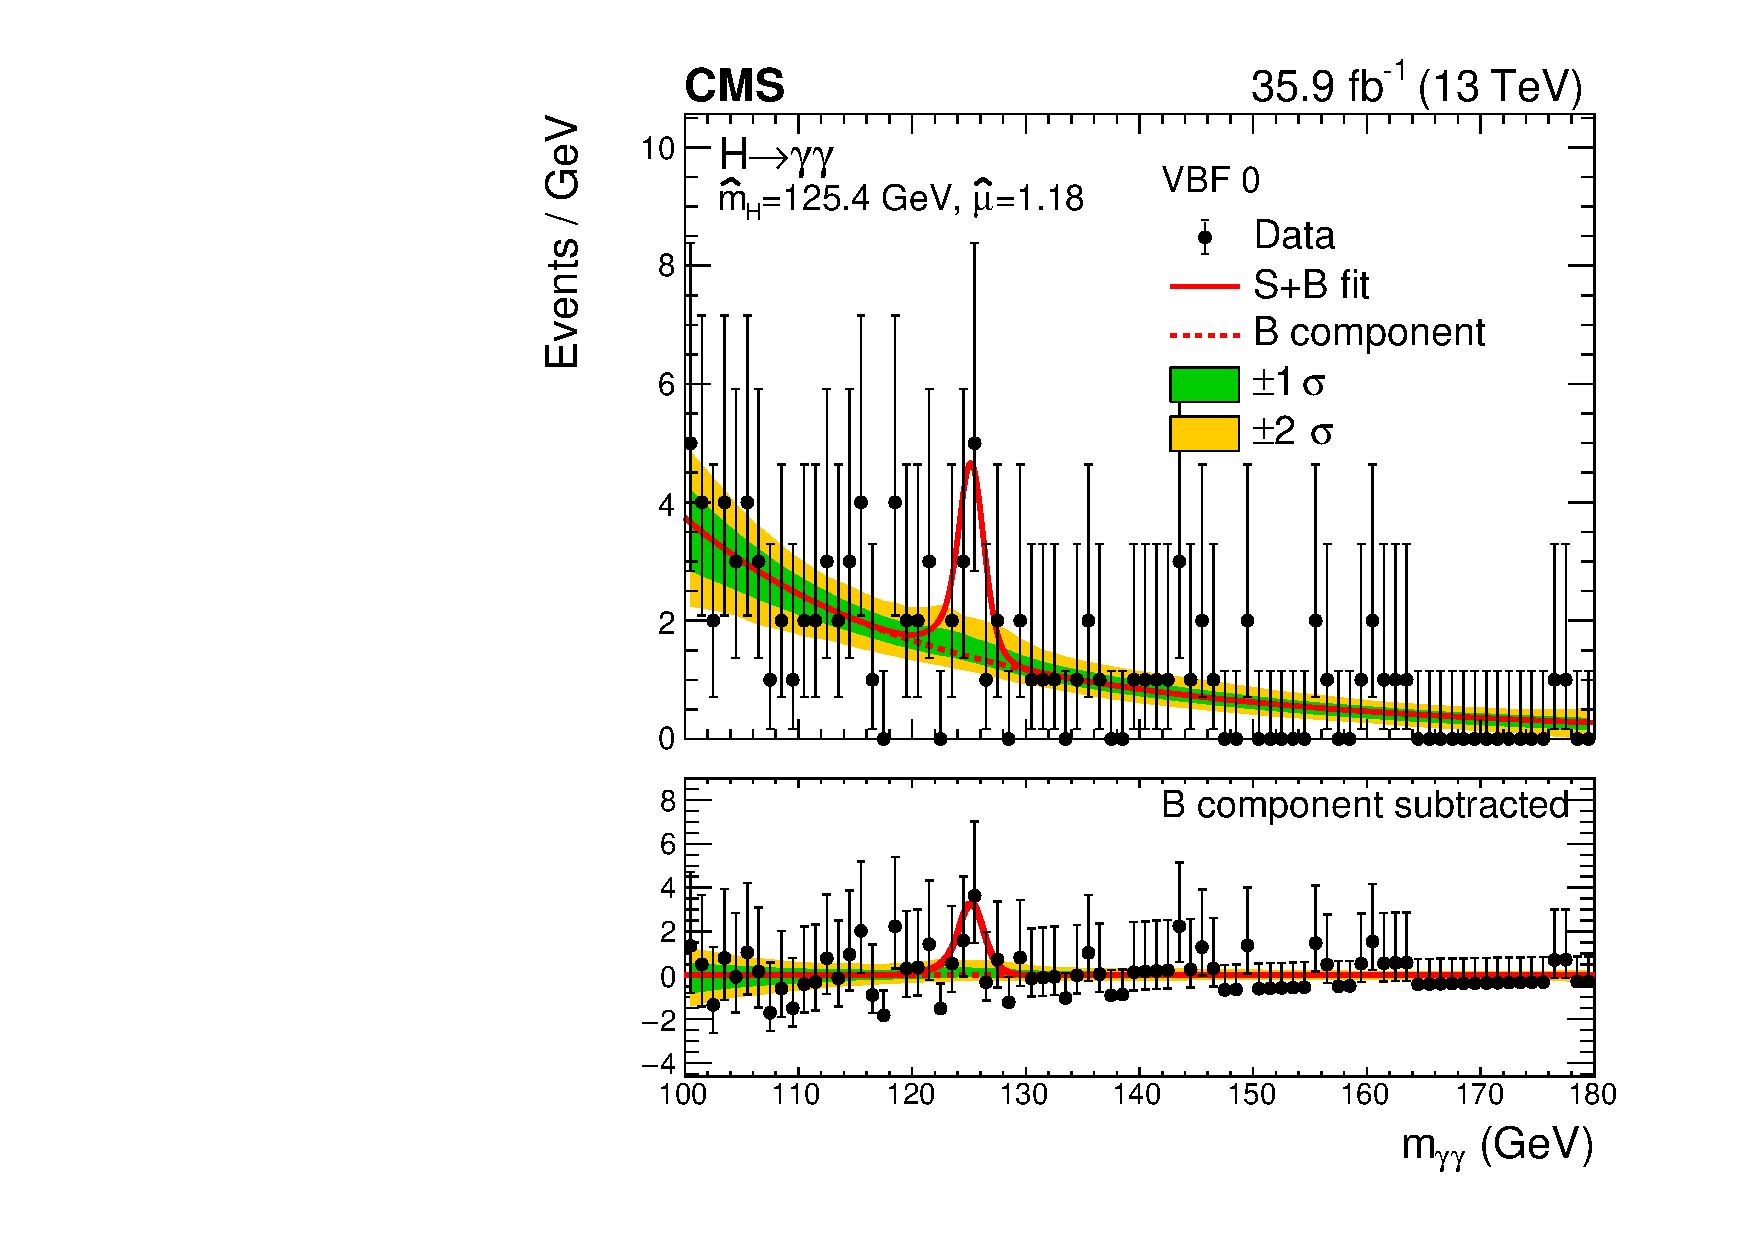
\includegraphics[width=0.47\textwidth]{figures/stats_results/CMS-HIG-16-040_Figure_012-a.pdf}
        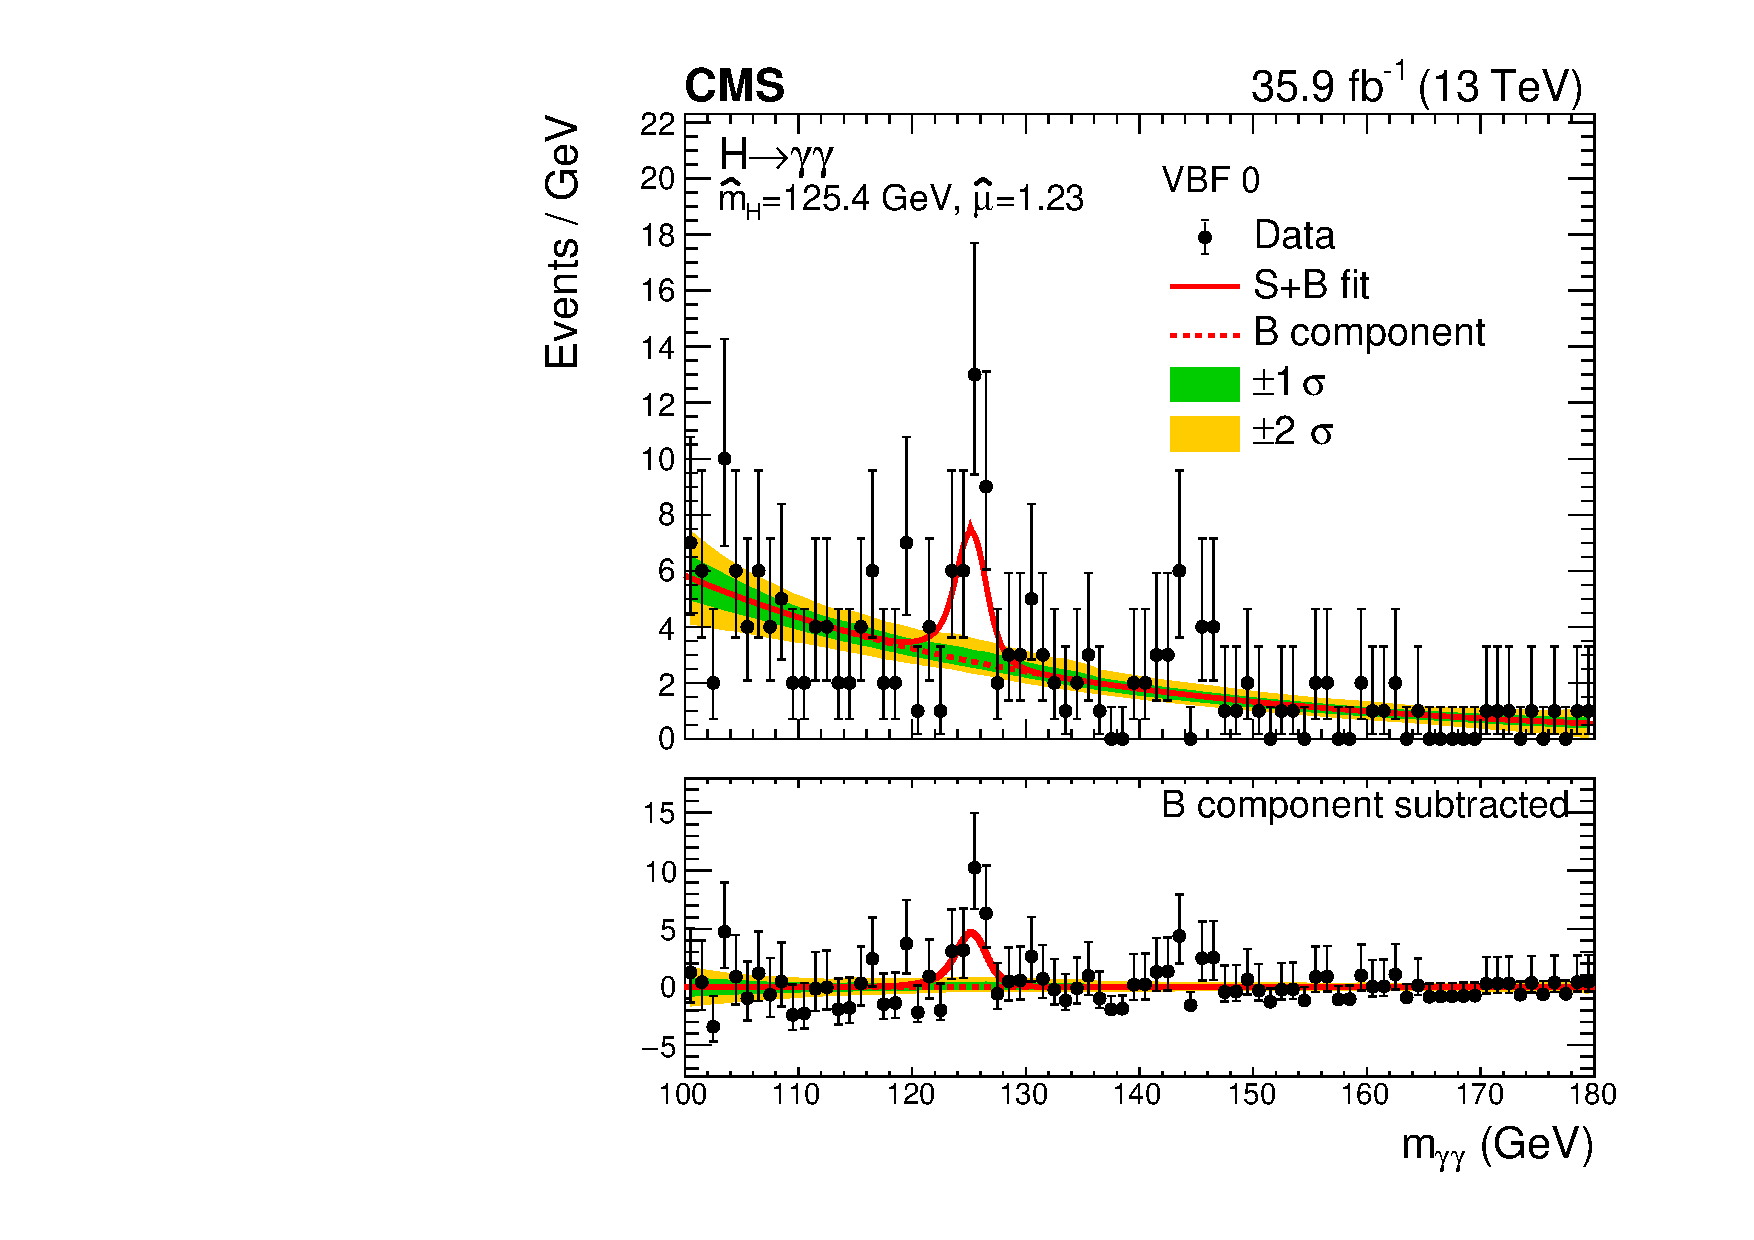
\includegraphics[width=0.47\textwidth]{figures/stats_results/SBplots_jackWSnewVBFTag_0_13TeV.pdf}
    \end{center}
    \begin{center}
        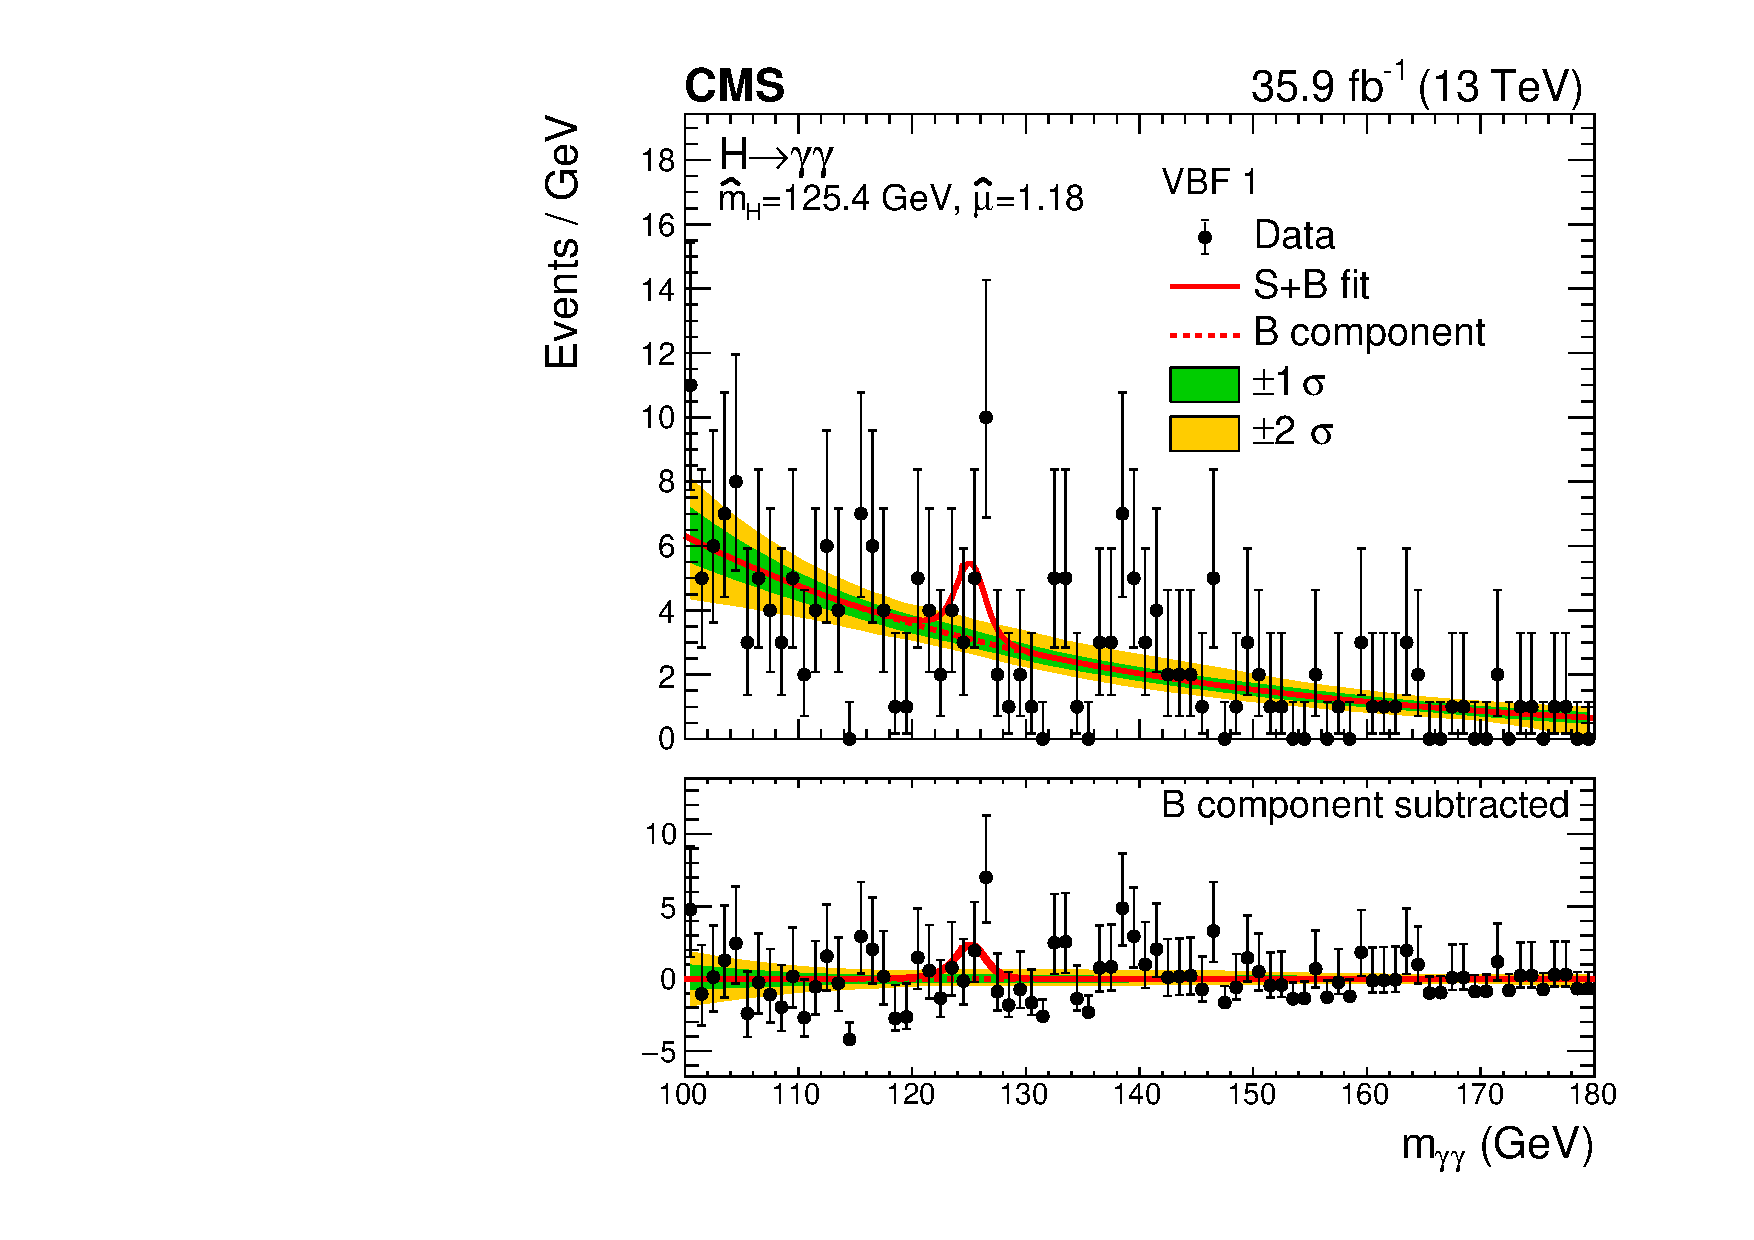
\includegraphics[width=0.47\textwidth]{figures/stats_results/CMS-HIG-16-040_Figure_012-b.pdf}
        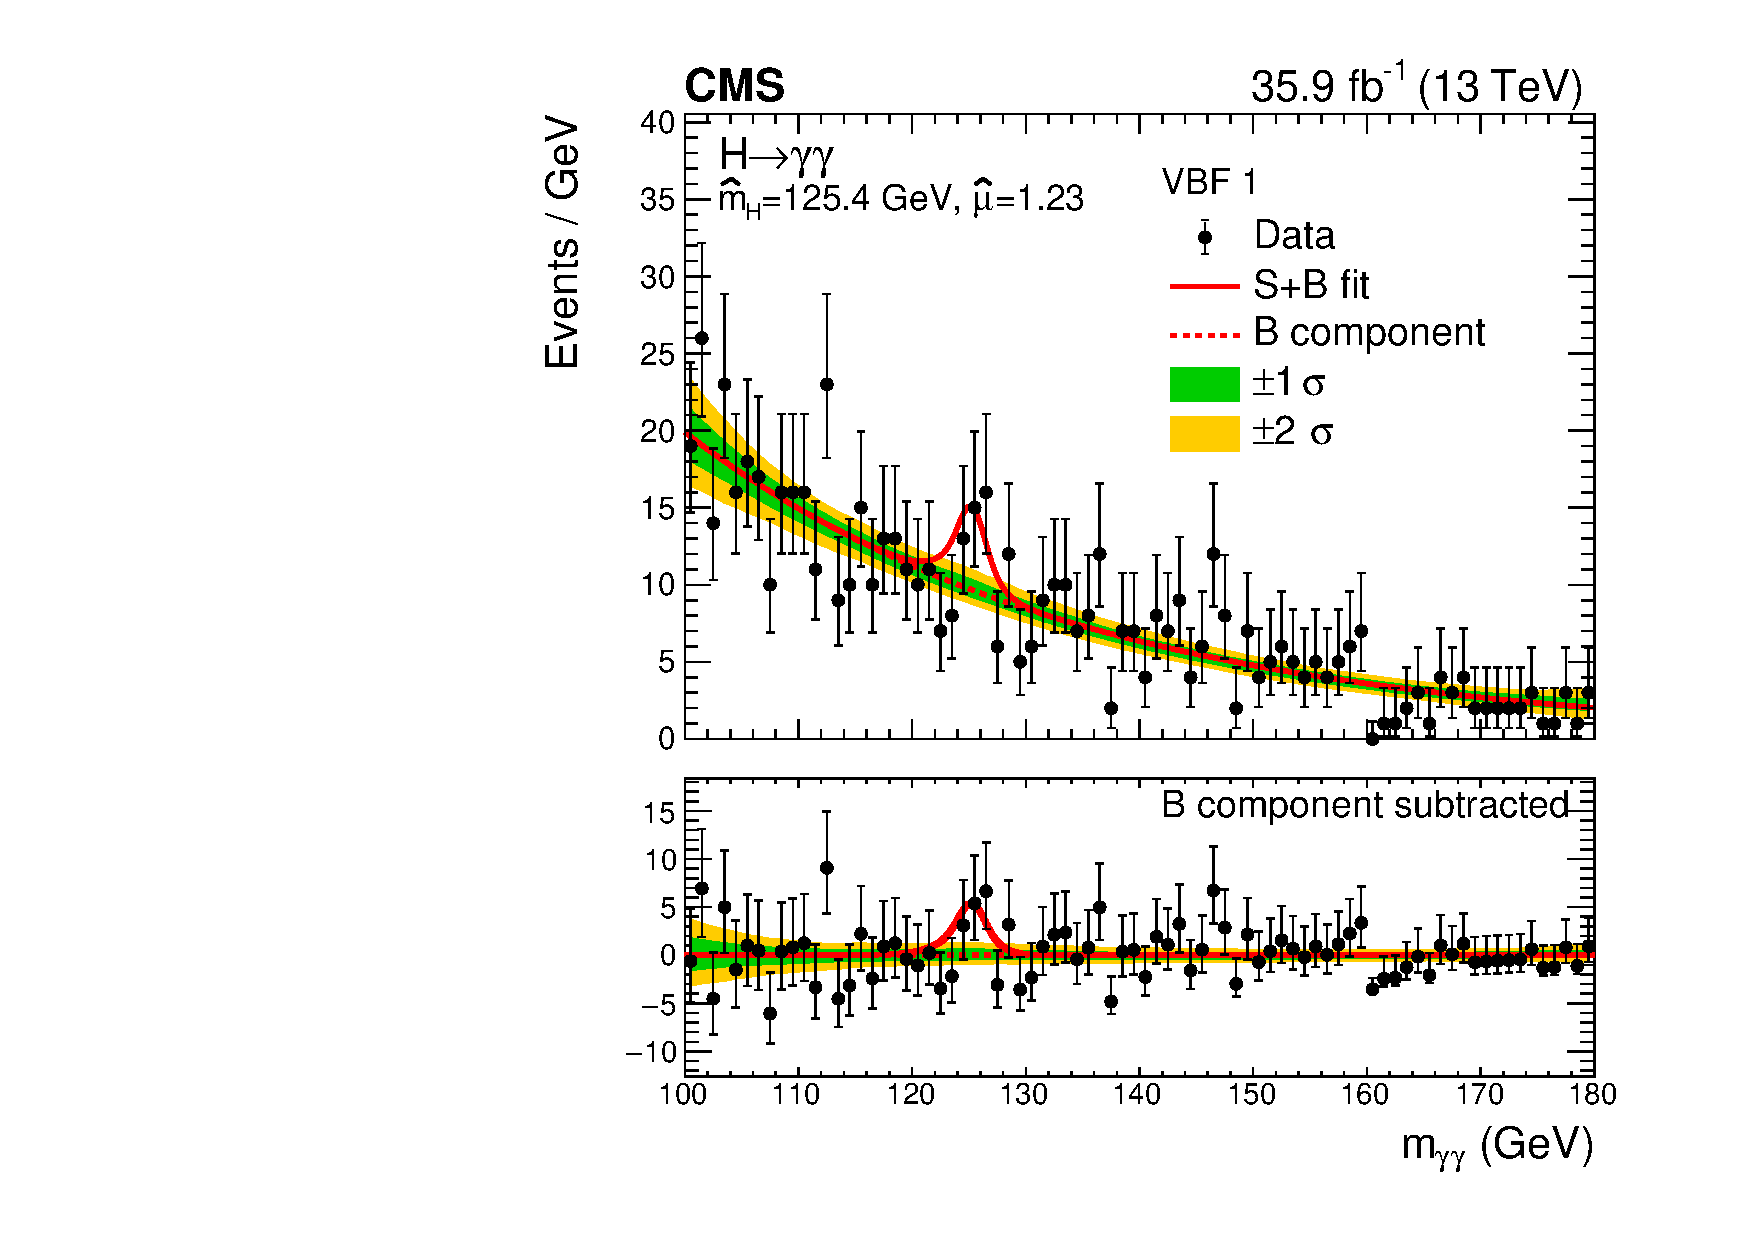
\includegraphics[width=0.47\textwidth]{figures/stats_results/SBplots_jackWSnewVBFTag_1_13TeV.pdf}
    \end{center}
    \begin{center}
        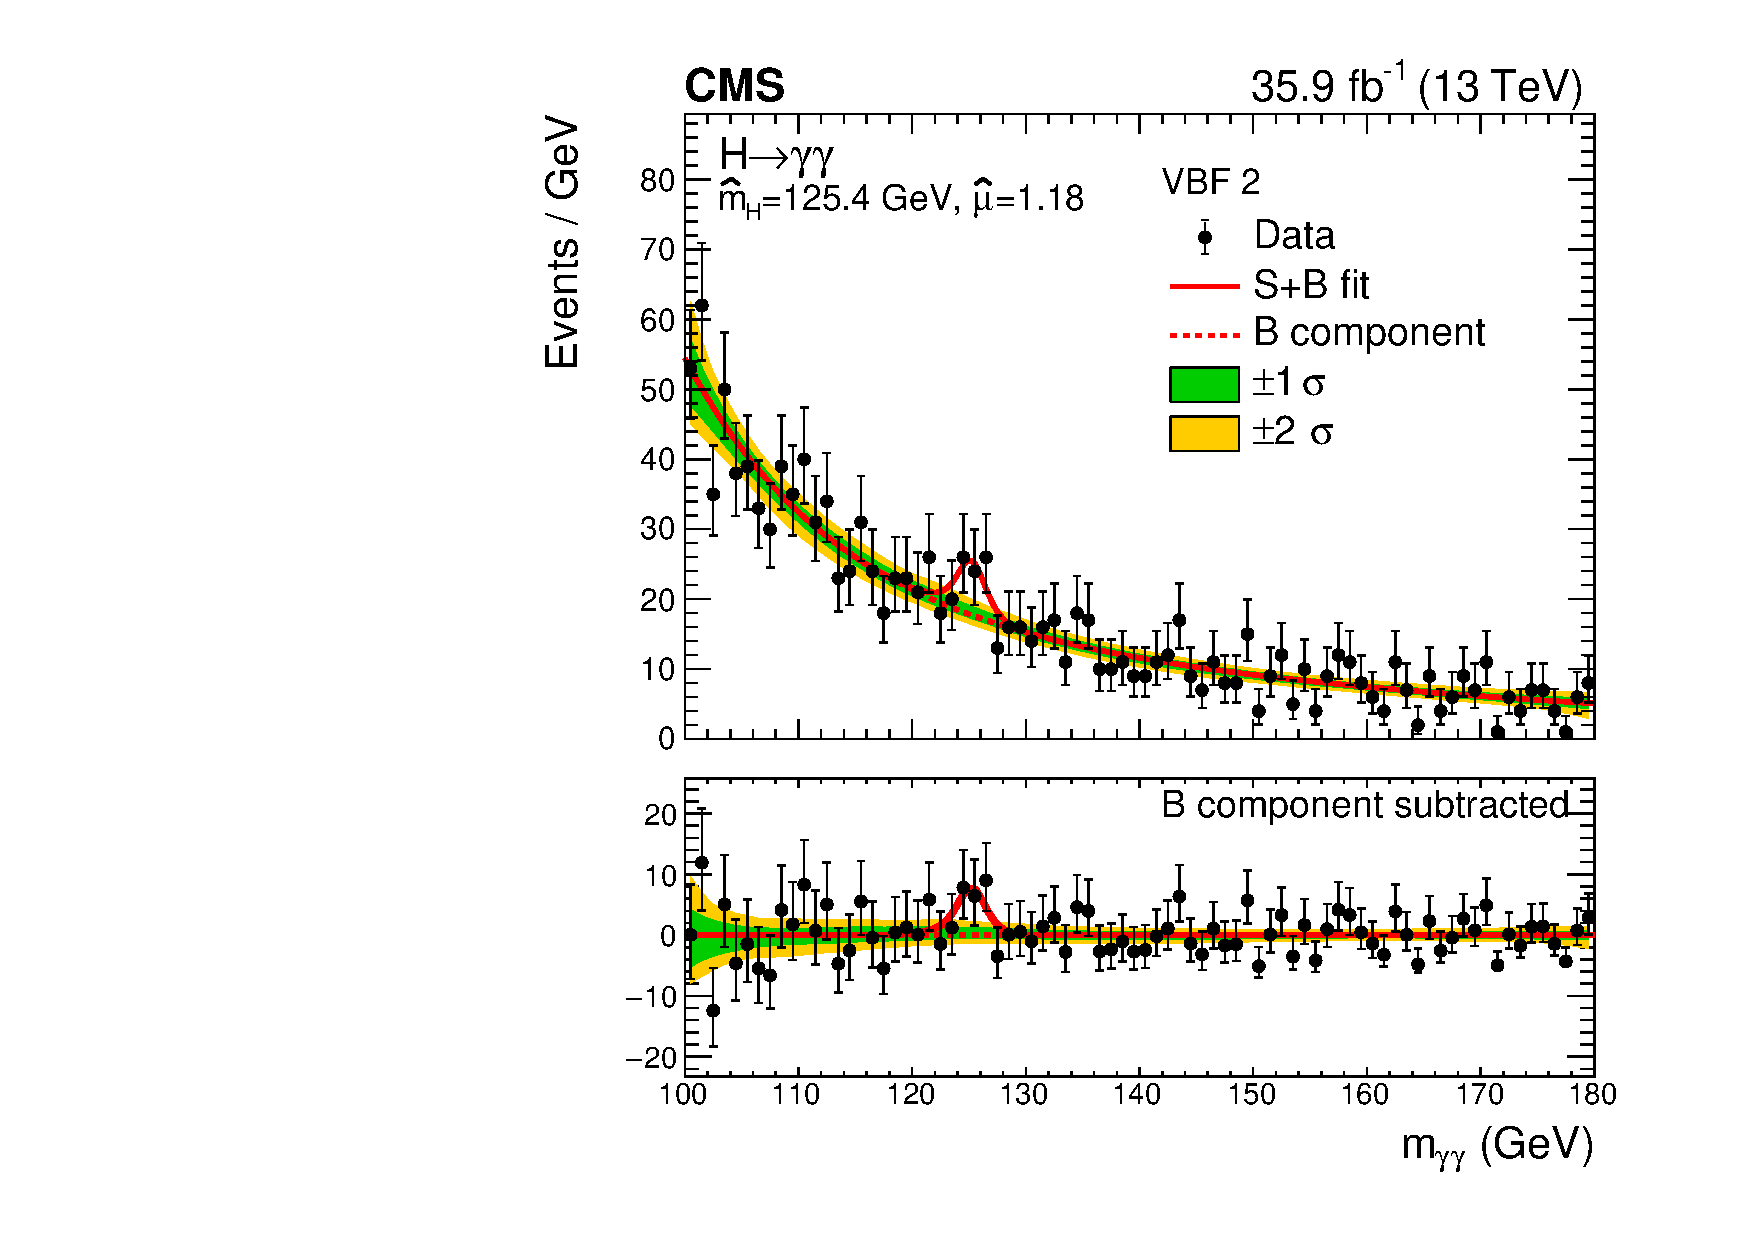
\includegraphics[width=0.47\textwidth]{figures/stats_results/CMS-HIG-16-040_Figure_012-c.pdf}
        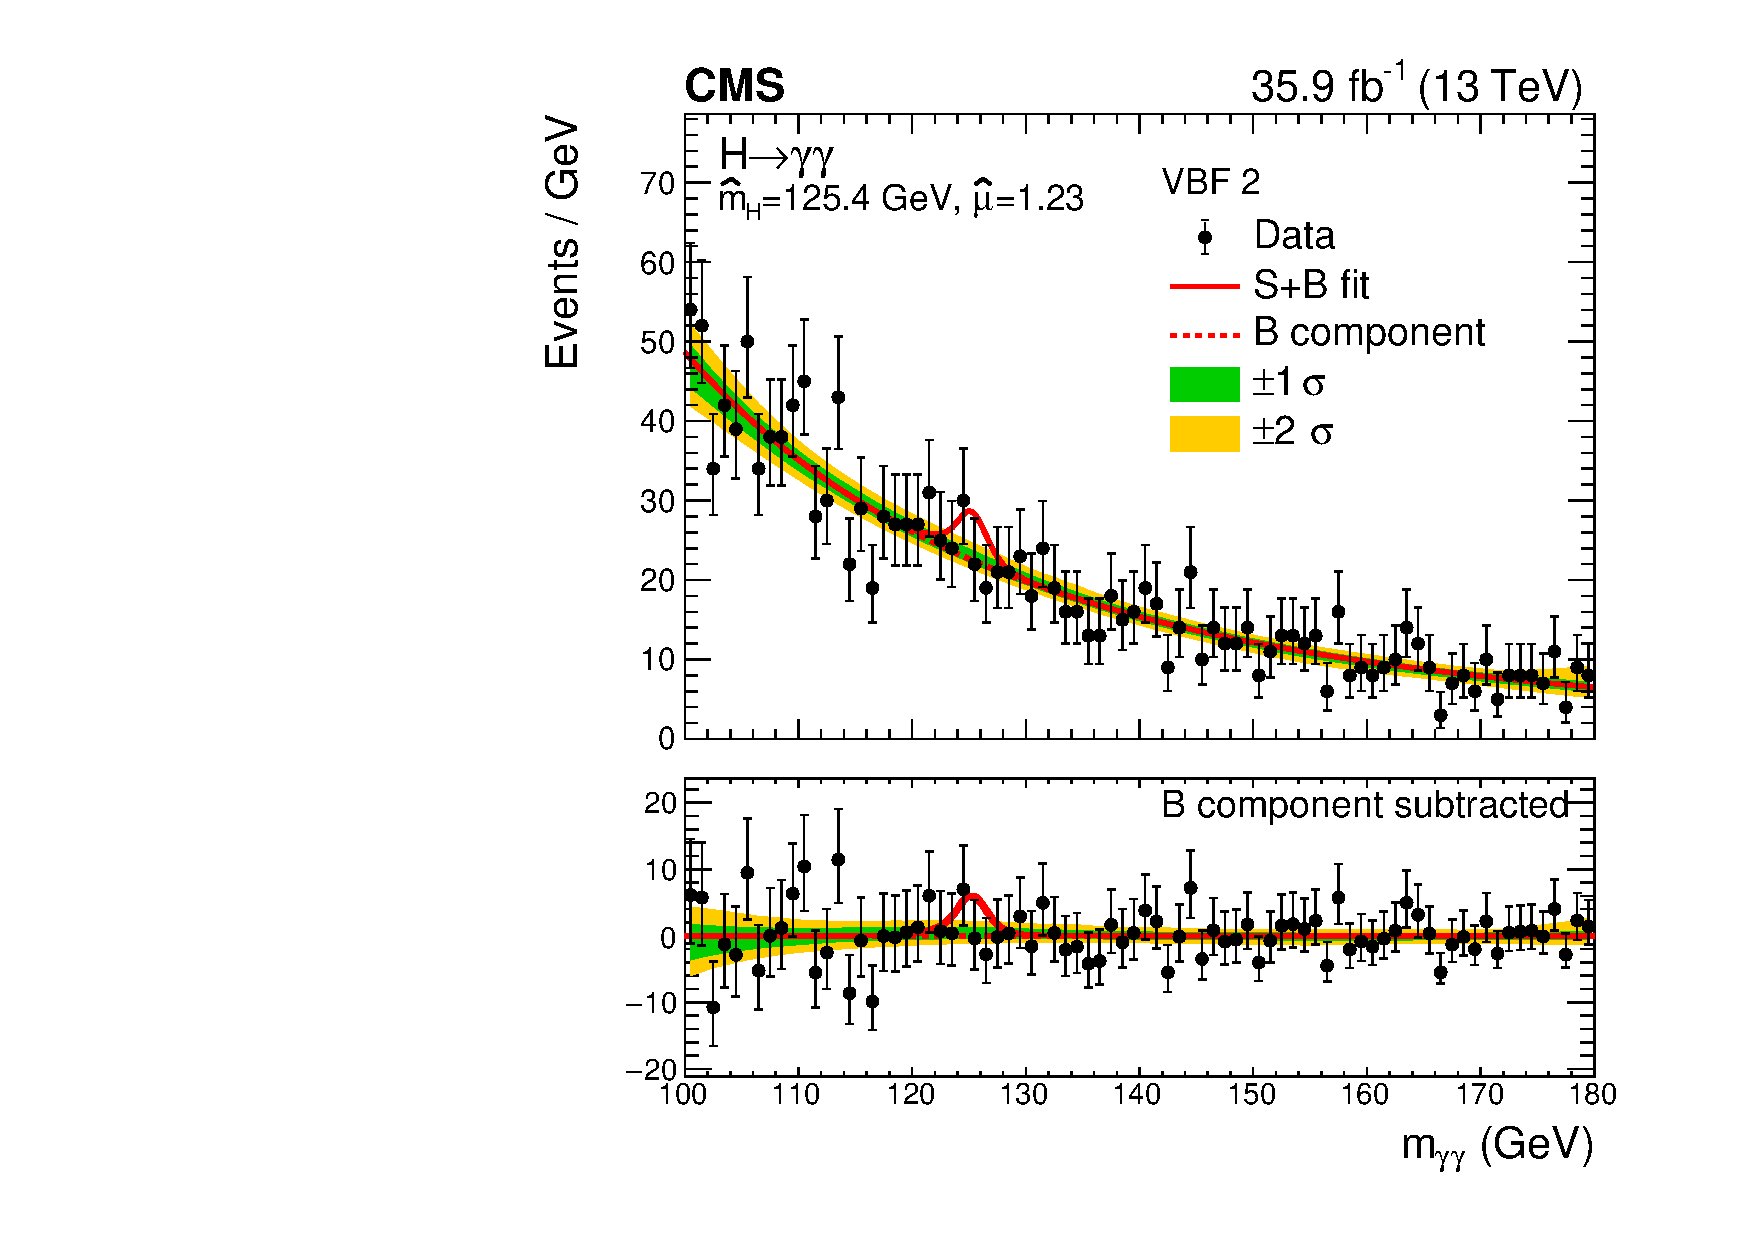
\includegraphics[width=0.47\textwidth]{figures/stats_results/SBplots_jackWSnewVBFTag_2_13TeV.pdf}
    \end{center}
    \caption{VBF category mass fits for the BDT-based VBF tag (left) and the DCNN-based VBF tag (right).
             Categories are shown in order from the most stringent to least: VBF 0 at the top to VBF 2 at the bottom.}
        \label{fig:stats_results:vbf_mass_plots}
\end{figure}


\begin{landscape}
    \begin{table}
        \centering
        \resizebox{1.5\textwidth}{!}{%
        \renewcommand{\arraystretch}{1.2}
        \begin{tabular}{rcccccccccccccc}
        \thickhline
            \multirow{2}{*}{Event categories} &\multicolumn{13}{c}{Expected SM 125\,GeV Higgs boson signal (BDT-based VBF tag)} & Bkg \\ \cline{2-14}
          &  Total & ggH & VBF & \ttH & bbH & tHq & tHW & WH lep & ZH lep & WH had & ZH had &   $\sigma_{\text{eff}}$  & $\sigma_{\text{HM}}$ & (GeV$^{-1}$) \\
          &  & & & & & & & & & & & (GeV) & (GeV) & \\
        \hline
        \rowcolor{GGH0} Untagged 0 &    32.5  &  72.0 \% &  16.6 \% &  2.6 \% &  0.6 \% &  0.7 \% &  0.3 \% &  0.6 \% &  0.3 \% &  4.2 \% &  2.2 \%& 1.32 & 1.26 & 21.8 \\
        \rowcolor{GGH1} Untagged 1 &    469.3  &  86.5 \% &  7.9 \% &  0.6 \% &  1.2 \% &  0.1 \% &  $<$0.05 \% &  0.5 \% &  0.3 \% &  1.9 \% &  1.1 \%& 1.46 & 1.32 & 925.1 \\
        \rowcolor{GGH2} Untagged 2 &    678.3  &  89.9 \% &  5.4 \% &  0.4 \% &  1.2 \% &  0.1 \% &  $<$0.05 \% &  0.5 \% &  0.3 \% &  1.4 \% &  0.8 \%& 1.93 & 1.67 & 2391.7 \\
        \rowcolor{GGH3} Untagged 3 &    624.3  &  91.3 \% &  4.4 \% &  0.5 \% &  1.0 \% &  0.1 \% &  $<$0.05 \% &  0.5 \% &  0.3 \% &  1.2 \% &  0.7 \%& 2.61 & 2.27 & 4855.1 \\
        \rowcolor{VBF0} VBF 0 &    9.3  &  15.5 \% &  83.2 \% &  0.4 \% &  0.4 \% &  0.3 \% &  $<$0.05 \% &  $<$0.05 \% &  $<$0.05 \% &  0.2 \% &  $<$0.05 \%& 1.52 & 1.31 & 1.6 \\
        \rowcolor{VBF1} VBF 1 &    8.0  &  28.4 \% &  69.7 \% &  0.4 \% &  0.6 \% &  0.4 \% &  $<$0.05 \% &  0.1 \% &  $<$0.05 \% &  0.3 \% &  0.1 \%& 1.66 & 1.38 & 3.3 \\
        \rowcolor{VBF2} VBF 2 &    25.2  &  45.1 \% &  51.2 \% &  0.9 \% &  0.8 \% &  0.6 \% &  0.1 \% &  0.2 \% &  0.1 \% &  0.8 \% &  0.3 \%& 1.64 & 1.37 & 18.9 \\
        \ttH Hadronic &    5.6  &  7.0 \% &  0.7 \% &  81.1 \% &  2.1 \% &  4.3 \% &  2.1 \% &  0.1 \% &  0.1 \% &  0.7 \% &  1.9 \%& 1.48 & 1.30 & 2.4 \\
        \ttH Leptonic &    3.8  &  1.5 \% &  $<$0.05 \% &  87.8 \% &  0.1 \% &  4.7 \% &  3.1 \% &  1.5 \% &  1.2 \% &  $<$0.05 \% &  $<$0.05 \%& 1.60 & 1.35 & 1.5 \\
        ZH Leptonic &    0.5  &  $<$0.05 \% &  $<$0.05 \% &  2.6 \% &  $<$0.05 \% &  $<$0.05 \% &  0.1 \% &  $<$0.05 \% &  97.3 \% &  $<$0.05 \% &  $<$0.05 \%& 1.65 & 1.43 & 0.1 \\
        WH Leptonic &    3.6  &  1.3 \% &  0.6 \% &  5.2 \% &  0.2 \% &  3.0 \% &  0.7 \% &  84.5 \% &  4.3 \% &  0.1 \% &  0.1 \%& 1.64 & 1.43 & 2.1 \\
        VH LeptonicLoose &    2.7  &  8.1 \% &  2.7 \% &  2.4 \% &  0.6 \% &  1.8 \% &  0.1 \% &  64.4 \% &  19.1 \% &  0.6 \% &  0.2 \%& 1.67 & 1.56 & 3.5 \\
        \rowcolor{VHH} VH Hadronic &    7.9  &  47.6 \% &  4.5 \% &  4.4 \% &  0.4 \% &  1.7 \% &  0.3 \% &  0.2 \% &  0.5 \% &  25.2 \% &  15.1 \%& 1.38 & 1.30 & 7.2 \\
        \rowcolor{VHM} VH MET &    4.0  &  18.7 \% &  2.6 \% &  15.4 \% &  0.4 \% &  2.1 \% &  1.2 \% &  26.8 \% &  30.4 \% &  1.4 \% &  0.9 \%& 1.56 & 1.39 & 3.5 \\
        \rowcolor{Gray} Total &    1875.0  &  86.9 \% &  7.1 \% &  1.0 \% &  1.1 \% &  0.2 \% &  $<$0.05 \% &  0.8 \% &  0.4 \% &  1.6 \% &  0.9 \%& 1.96 & 1.62 & 8237.8 \\
        \hline
            \multirow{2}{*}{} &\multicolumn{13}{c}{Expected SM 125\,GeV Higgs boson signal (DCNN-based VBF tag and Downstream Tags)} & \\ \cline{2-14}
        \hline
        \rowcolor{GGH0} Untagged 0 &    33.3  &  73.5 \% &  14.7 \% &  2.9 \% &  0.6 \% &  0.7 \% &  0.3 \% &  0.6 \% &  0.3 \% &  4.2 \% &  2.2 \%& 1.26 & 1.19 &  21.7 \\
        \rowcolor{GGH1} Untagged 1 &    466.5  &  87.2 \% &  7.3 \% &  0.6 \% &  1.2 \% &  0.1 \% &  $<$0.05 \% &  0.5 \% &  0.3 \% &  1.8 \% &  1.1 \%& 1.46 & 1.31 &  910.0 \\
        \rowcolor{GGH2} Untagged 2 &    674.8  &  90.3 \% &  5.0 \% &  0.4 \% &  1.2 \% &  0.1 \% &  $<$0.05 \% &  0.5 \% &  0.3 \% &  1.4 \% &  0.8 \%& 1.92 & 1.64 &  2415.6 \\
        \rowcolor{GGH3} Untagged 3 &    620.5  &  91.6 \% &  4.1 \% &  0.5 \% &  1.0 \% &  0.1 \% &  $<$0.05 \% &  0.5 \% &  0.3 \% &  1.2 \% &  0.7 \%& 2.62 & 2.29 &  4848.2 \\
        \rowcolor{VBF0} VBF 0 &    14.2  &  9.5 \% &  89.7 \% &  0.2 \% &  0.3 \% &  0.2 \% &  $<$0.05 \% &  0.1 \% &  $<$0.05 \% &  0.1 \% &  $<$0.05 \%& 1.70 & 1.41 &  3.4 \\
        \rowcolor{VBF1} VBF 1 &    17.2  &  25.0 \% &  73.2 \% &  0.3 \% &  0.5 \% &  0.4 \% &  $<$0.05 \% &  0.1 \% &  $<$0.05 \% &  0.3 \% &  0.1 \%& 1.78 & 1.43 & 10.6 \\
        \rowcolor{VBF2} VBF 2 &    19.6  &  44.2 \% &  51.7 \% &  0.7 \% &  0.9 \% &  0.6 \% &  $<$0.05 \% &  0.2 \% &  $<$0.05 \% &  1.2 \% &  0.5 \%& 1.78 & 1.40 & 23.0 \\
        \rowcolor{VHH} VH Hadronic &    7.9  &  47.3 \% &  4.5 \% &  4.8 \% &  0.4 \% &  1.7 \% &  0.3 \% &  0.3 \% &  0.5 \% &  25.2 \% &  14.9 \%& 1.46 & 1.38 & 7.2 \\
        \rowcolor{VHM} VH MET &    3.9  &  19.0 \% &  3.0 \% &  13.4 \% &  0.5 \% &  2.2 \% &  1.2 \% &  27.3 \% &  30.9 \% &  1.5 \% &  1.0 \%& 1.61 & 1.46 & 3.4 \\
        \rowcolor{Gray} Total &    1874.3  &  86.9 \% &  7.1 \% &  1.0 \% &  1.1 \% &  0.1 \% &  $<$0.05 \% &  0.8 \% &  0.4 \% &  1.6 \% &  0.9 \%& 1.96 & 1.61 & 8252.9 \\
        \thickhline
        \end{tabular}%
    }
        \caption{Expected signal yields per category for the BDT-based VBF tag (top) and the DCNN-based VBF tag (bottom). 
                 Only the downstream tags are shown for the DCNN-based tag as the others are unaffected.
                 The width values $\sigma_{\text{eff}}$ and $\sigma_{\text{HM}}$ correspond to the smallest interval 
                 containing 68.3\% of the \mgg distribution and the width at half maximum of the signal peak respectively.}
        \label{tab:stats_results:yield_table}
    \end{table}
\end{landscape}
\begin{table}[h!]
    \centering
    \renewcommand{\arraystretch}{1.3}
    \begin{tabular}{r|cccc}
        \thickhline
        & \multicolumn{4}{c}{$S/\sqrt{S+B}$} \\ 
        VBF tag & VBF 0 & VBF 1 & VBF 2 & Total \\
        \hline
        BDT-based  & 2.02 & 1.25 & 1.35 & 2.73\\
        DCNN-based & 2.44 & 1.65 & 0.97 & 3.10\\
        \thickhline
    \end{tabular}
    \caption{VBF tag category expected signal significances comparing the BDT-based VBF tag to the DCNN-based VBF tag.}
    \label{tab:stats_results:sig_table}
\end{table}



The final combined mass plots for both unweighted and weighted by sensitivity are shown in Figure \ref{fig:stats_results:comb_mass_plots}. The change to a DCNN-based VBF tag does not have a significant effect on these plots.
\begin{figure}[h!]
    \begin{center}
        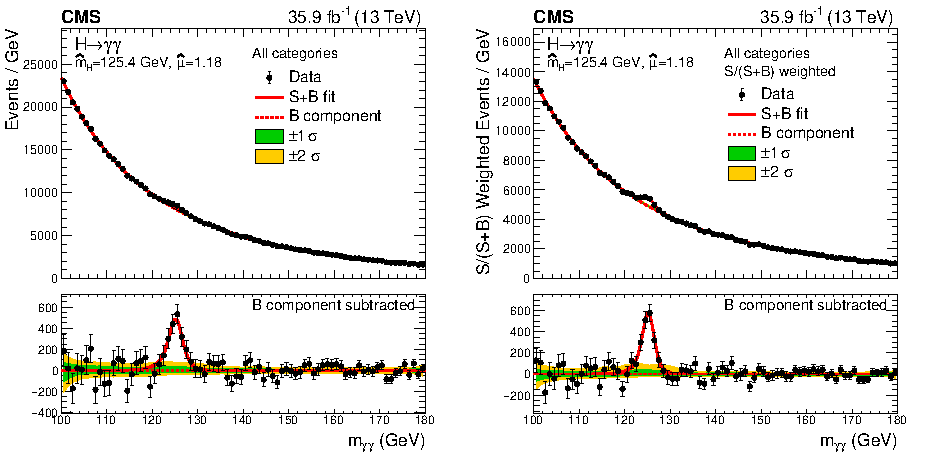
\includegraphics[width=1.0\textwidth]{figures/stats_results/CMS-HIG-16-040_Figure_014.pdf}
    \end{center}
    \caption{Diphoton mass distribution plots for all categories combined using the BDT-based VBF tag.
            The unweighted combined distribution is shown on the left, and the sensitivity weighted combination is shown on the right.}
        \label{fig:stats_results:comb_mass_plots}
\end{figure}








\subsection{Signal Strength Likelihood Scans}
The test statistic used is the twice-negative delta log-likelihood ($2\Delta{\mathrm{NLL}}$), 
\begin{equation}
    2\Delta{\mathrm{NLL}} = -2\ln{\mathcal{L}}(\mu,\hat{m}_{H,\mu},\vec{n}_{\mu} | m_{\gamma\gamma}) + 2\ln\mathcal{L}(\hat{\mu},\hat{m}_{H},\hat{n} | m_{\gamma\gamma}),
\end{equation}
where $\hat{\mu}$, $\hat{m}_{H}$ and $\hat{n}$ are the best fit values for the signal strength modifier, Higgs mass and nuisance parameters respectively. 
The parameters $\mu$, $\hat{m}_{H,\mu}$ and $\vec{n}_{\mu}$ are the global signal strength being profiled in the likelihood scan, the Higgs mass allowed to float for a given value of $\mu$, and the nuisance parameter values also allowed to float. 

This procedure is used to measure the global $\mu$, the production mode $\mu$ values and the fermionic versus bosonic production $\mu$ values. 

\subsubsection{Global Signal Strength Likelihood Scan}
To calculate the uncertainty associated with the measurement of the global signal strength a likelihood scan is performed with a test statistic and profiling in the value of $\mu$.
The contribution of statistical uncertainty is determined by performing the likelihood scan with the nuisance parameters associated with systematic uncertainties removed. 
The systematic contribution is then the difference in quadrature between these values and the total uncertainty from the full fit. 
The $2\Delta{\mathrm{NLL}}$ values of the global $\mu$ likelihood scans are shown in Figure \ref{fig:stats_results:global_mu_scan}.
\begin{figure}[h!]
    \begin{center}
        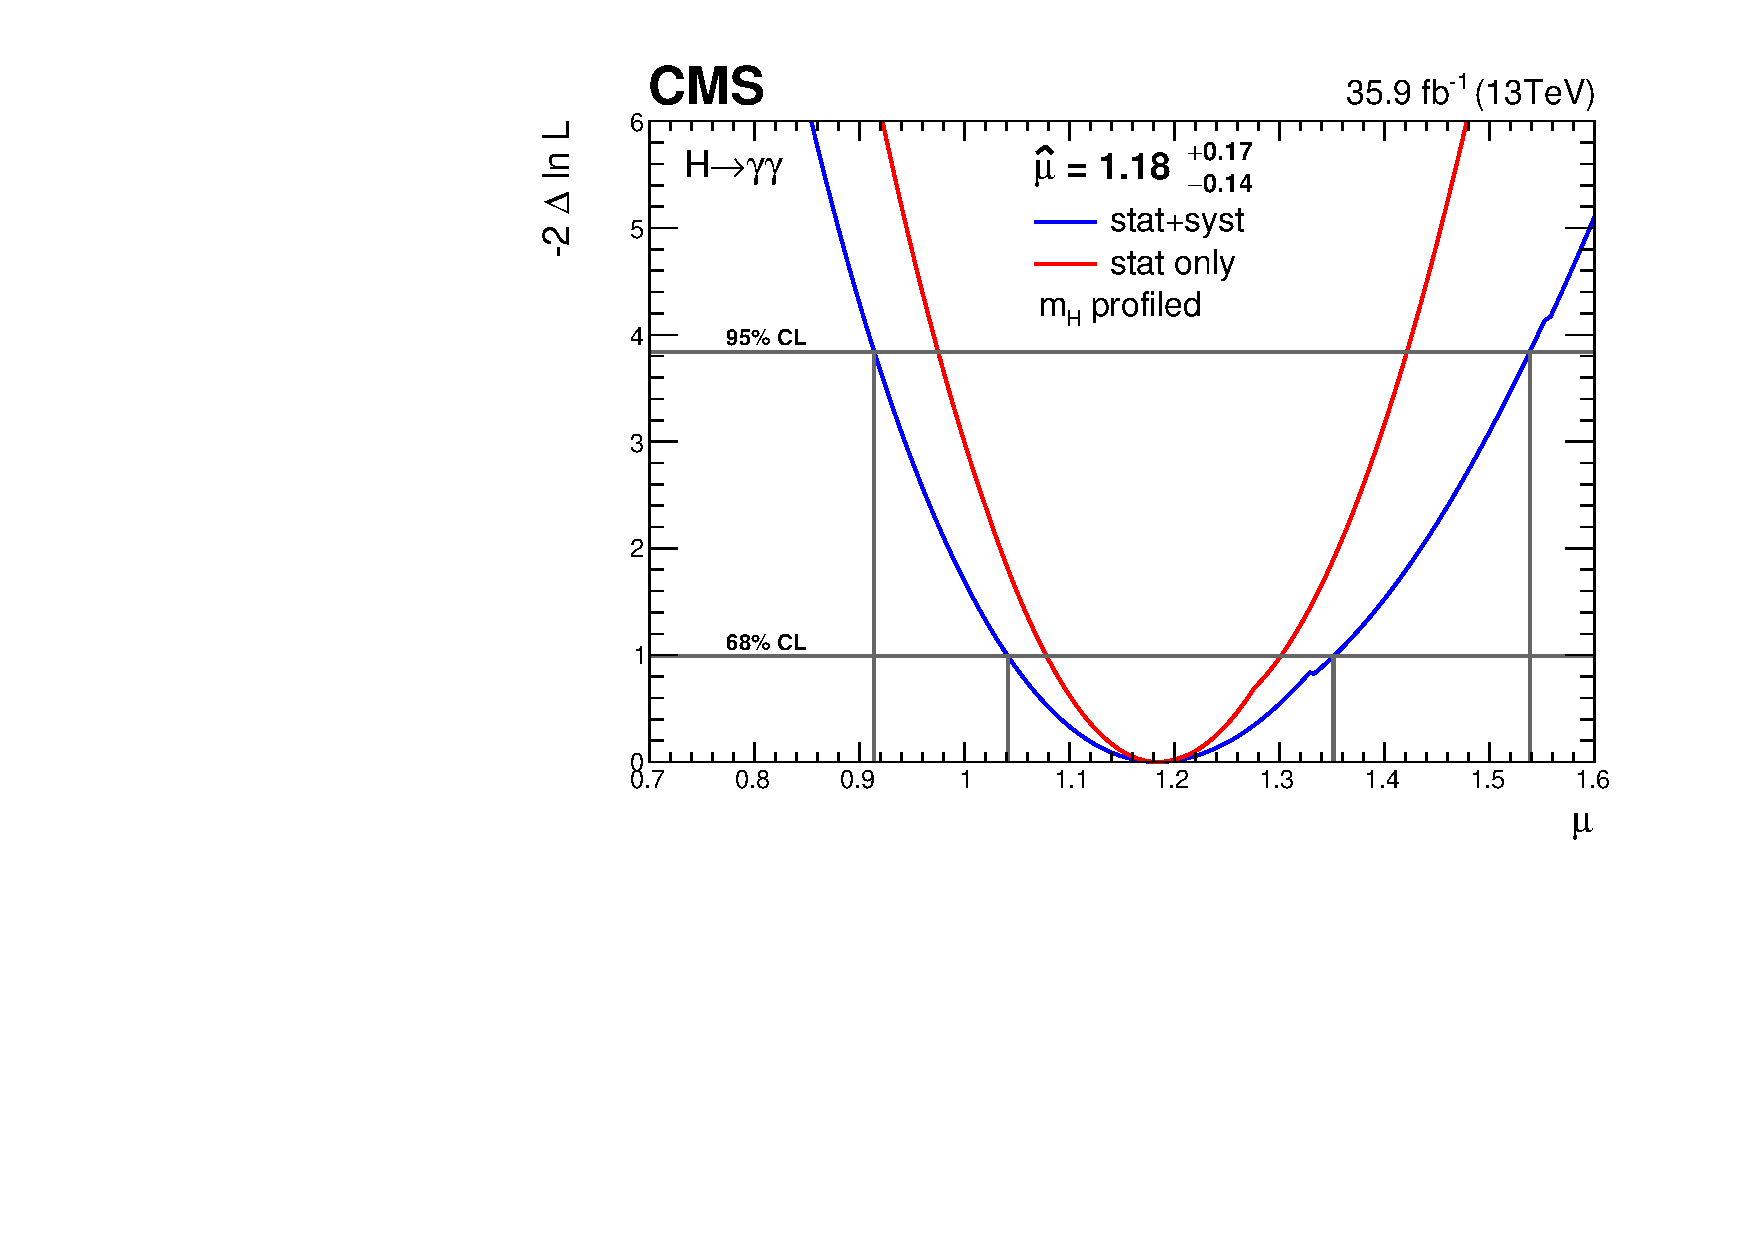
\includegraphics[width=0.6\textwidth]{figures/stats_results/CMS-HIG-16-040_Figure_016.pdf}
        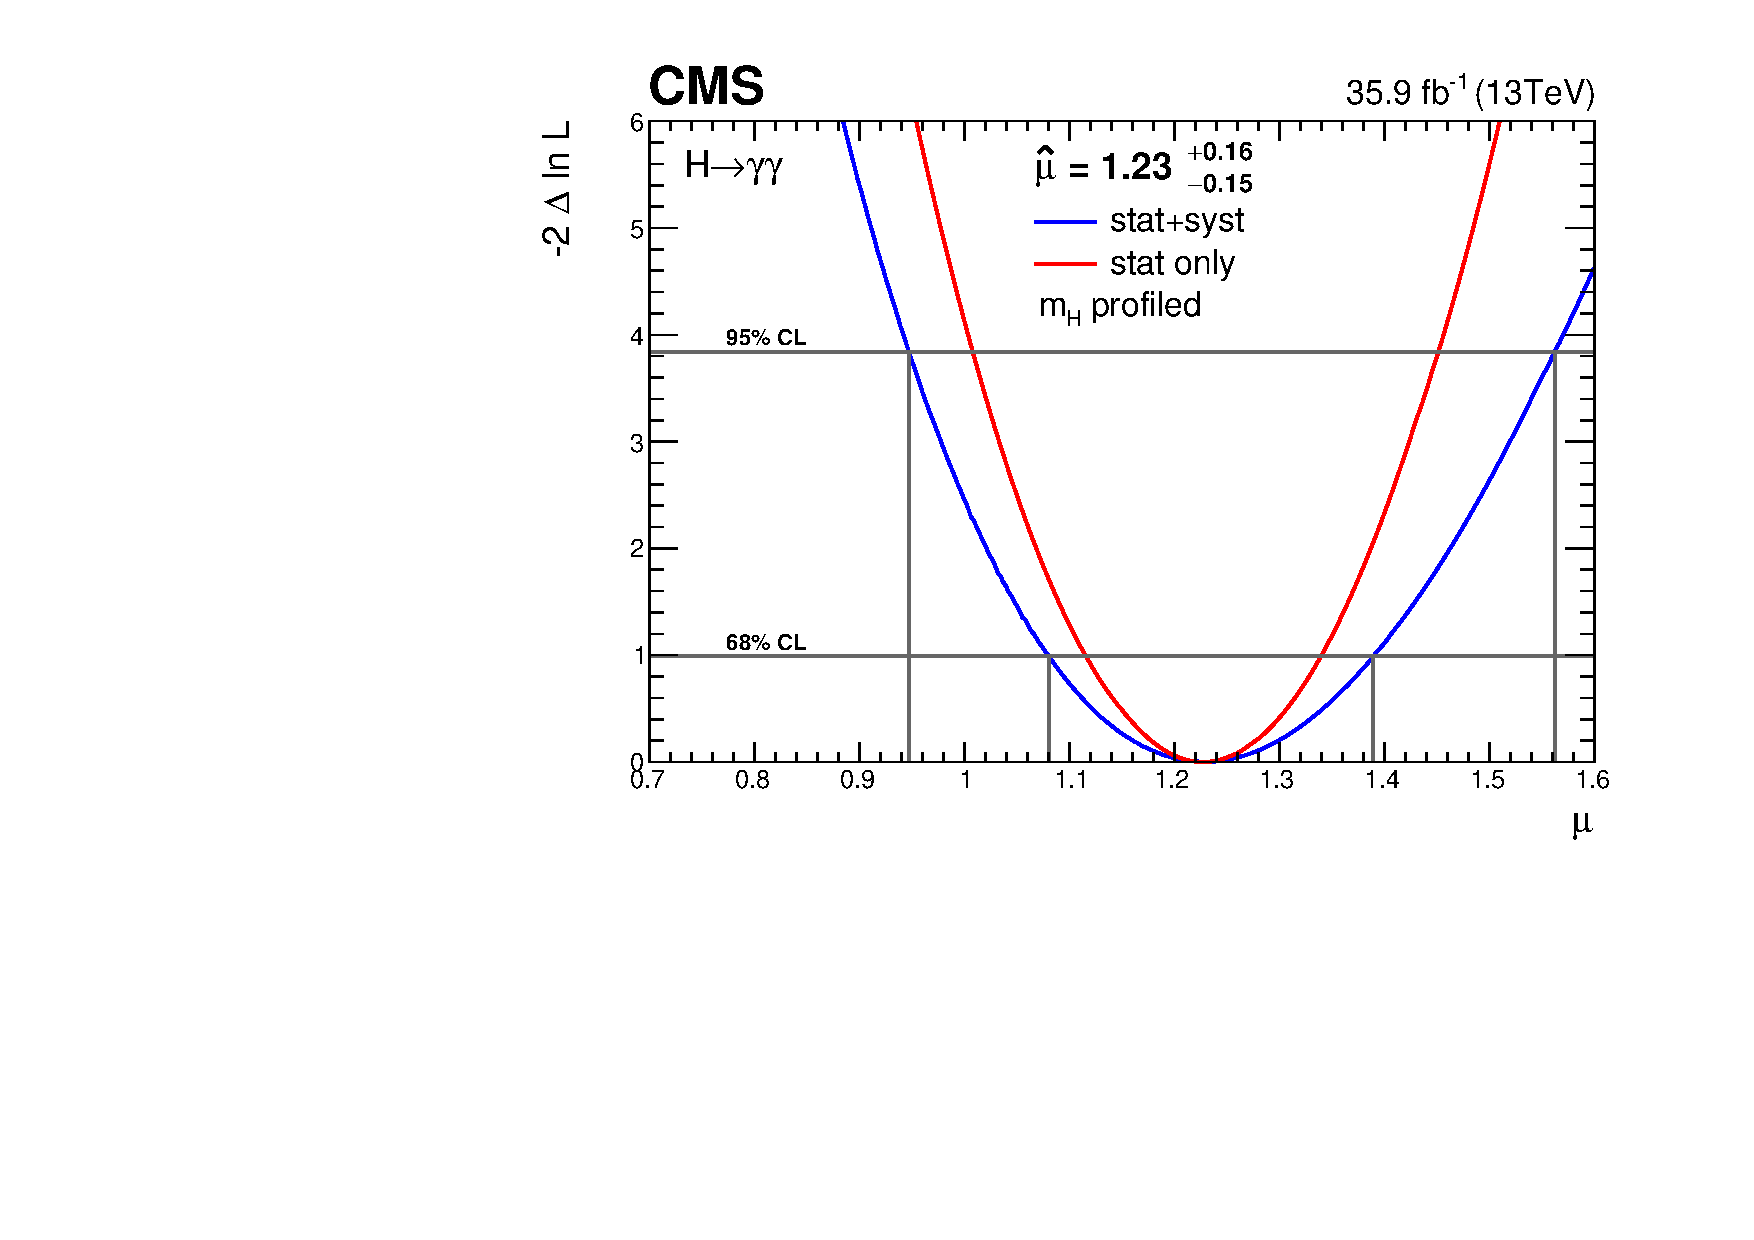
\includegraphics[width=0.6\textwidth]{figures/stats_results/MuScanProfileMH.pdf}
    \end{center}
    \caption{Likelihood scan of the global signal strength modifier $\mu$ with a $2\Delta{\mathrm{NLL}}$ test statistic for analysis with the BDT-based VBF tag (top) and the DCNN-based VBF tag (bottom).}
        \label{fig:stats_results:global_mu_scan}
\end{figure}

The measured value for $\mu$ and its associated uncertainties in the BDT-based case are found to be $\hat{\mu} = 1.18^{+0.17}_{-0.14} = 1.18^{+0.12}_{-0.11}(\mathrm{stat.})^{+0.09}_{-0.07}(\mathrm{syst.})^{+0.07}_{-0.06}(\mathrm{theo.})$.
The best fit value for the Higgs boson mass is found to be $\hat{m}_{H}=125.4\pm{0.3}=125.4\pm{0.2}(\mathrm{stat}.)\pm{0.2}(\mathrm{syst}.)$. 
A precise determination of the systematic effects on the mass value and therefore a precise determination of the mass itself are beyond the scope of this thesis.

The measured value for $\mu$ is found to be larger in the DCNN case with similar-sized uncertainties: $\hat{\mu} = 1.24^{+0.16}_{-0.15} = 1.24^{+0.11}_{-0.11}(\mathrm{stat.})^{+0.08}_{-0.08}(\mathrm{syst.})^{+0.06}_{-0.07}(\mathrm{theo.})$.
The best fit value for the Higgs boson mass is unchanged. 














\subsubsection{Production Mode Signal Strength Modifiers}
Likelihood scans specific to each production mode are carried out in a similar way to the global case, but with some differences. 
Instead of a single global $\mu$ and likelihood scan there are four, one for each production mode. 
For each case the corresponding $\mu$ is profiled and the others are allowed to float in the fit. 
The results of these likelihood scans are shown in Figure \ref{fig:stats_results:prod_mu_scans}. 
\begin{figure}[h!]
    \begin{center}
        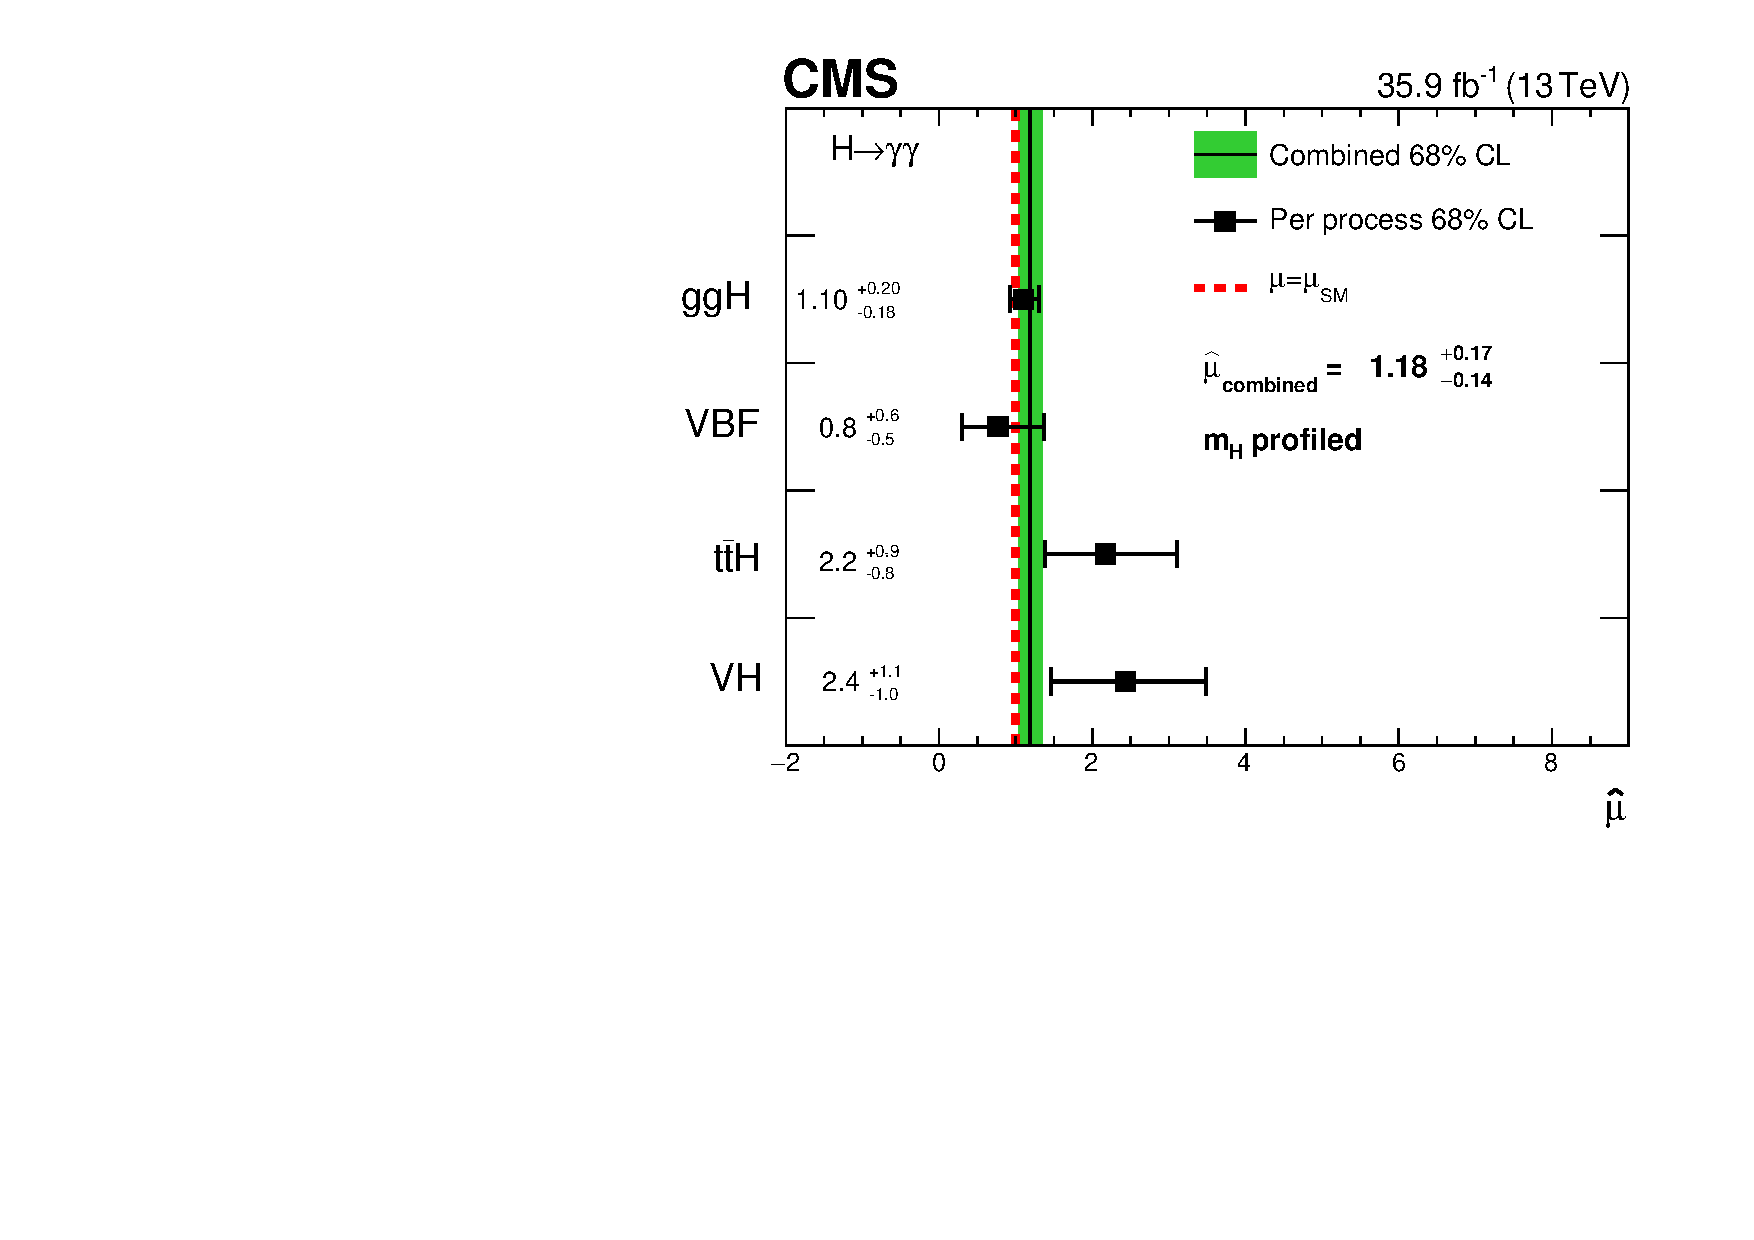
\includegraphics[width=0.75\textwidth]{figures/stats_results/CMS-HIG-16-040_Figure_017.pdf}
        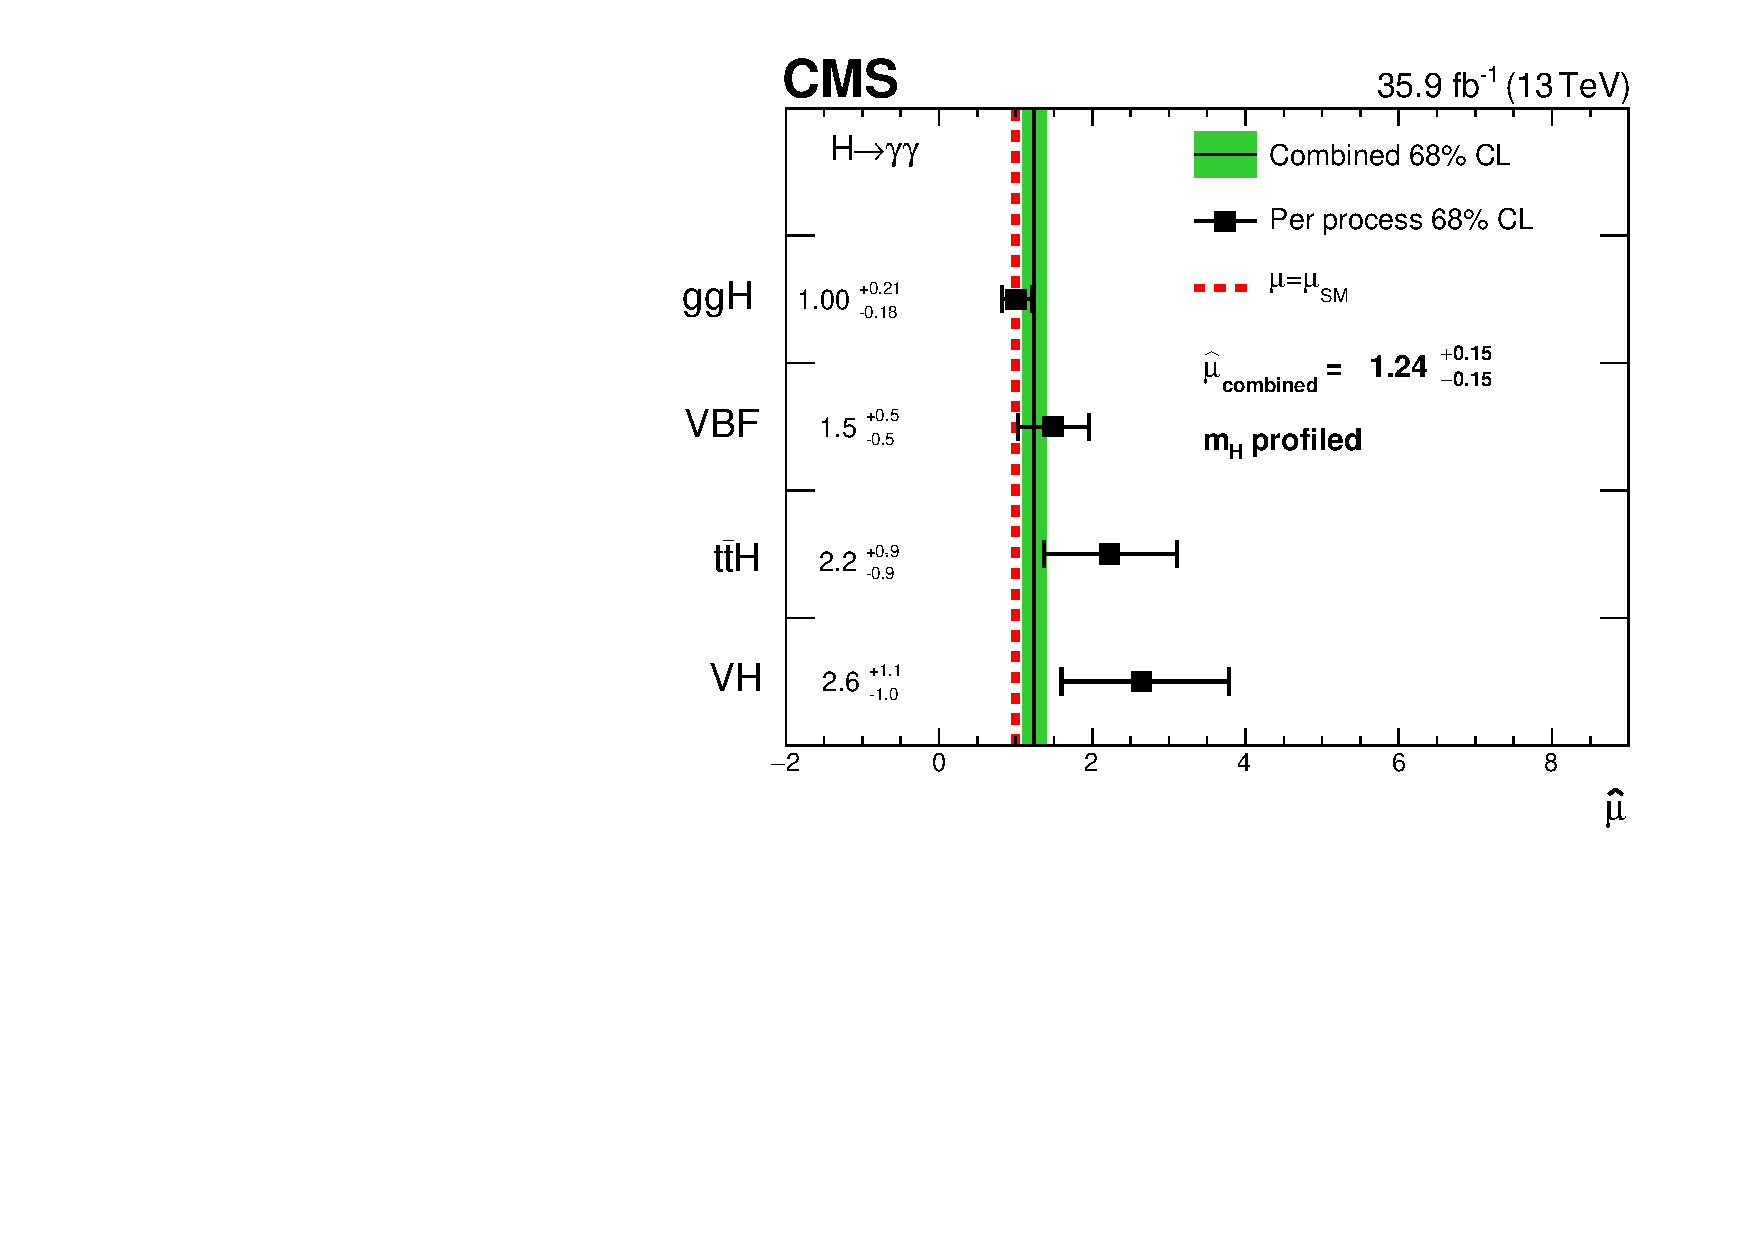
\includegraphics[width=0.75\textwidth]{figures/stats_results/PerProcessMuProfileMH.pdf}
    \end{center}
    \caption{Likelihood scan results of the production mode signal strength modifiers $\mu$ with a $2\Delta{\mathrm{NLL}}$ test statistic. Analysis with the BDT-based VBF tag is shown at the top and the DCNN-based variant is at the bottom.}
        \label{fig:stats_results:prod_mu_scans}
\end{figure}

The DCNN-based VBF tag leads to a change in the VBF measurement from $\mu_{\mathrm{VBF}}=0.8^{+0.6}_{-0.5}$ to $\mu_{\mathrm{VBF}}=1.5^{+0.5}_{-0.5}$.
The measured signal strength has increased, and there has been a small reduction in the uncertainty of its measurement.
The other production modes are mostly unchanged except for the ggH and VH which correspond to tags downstream from VBF.


The same approach is used to extract the ratio of observed cross sections to the SM expectation as part of the simplified template cross section (STXS) framework Stage 0 \cite{LHCHXS}.
This scheme is aimed at reducing the impact of theory uncertainties due to extrapolation to the full phase space from the fiducial region of the analysis. 
This imposes a criterion on the Higgs boson rapidity of $y<2.5$ and splits the VH into separate WH, ZH and VH Hadronic categories. 
The results of measuring these ratios are shown in Figure \ref{fig:stats_results:stxs}.
\begin{figure}[h!]
    \begin{center}
        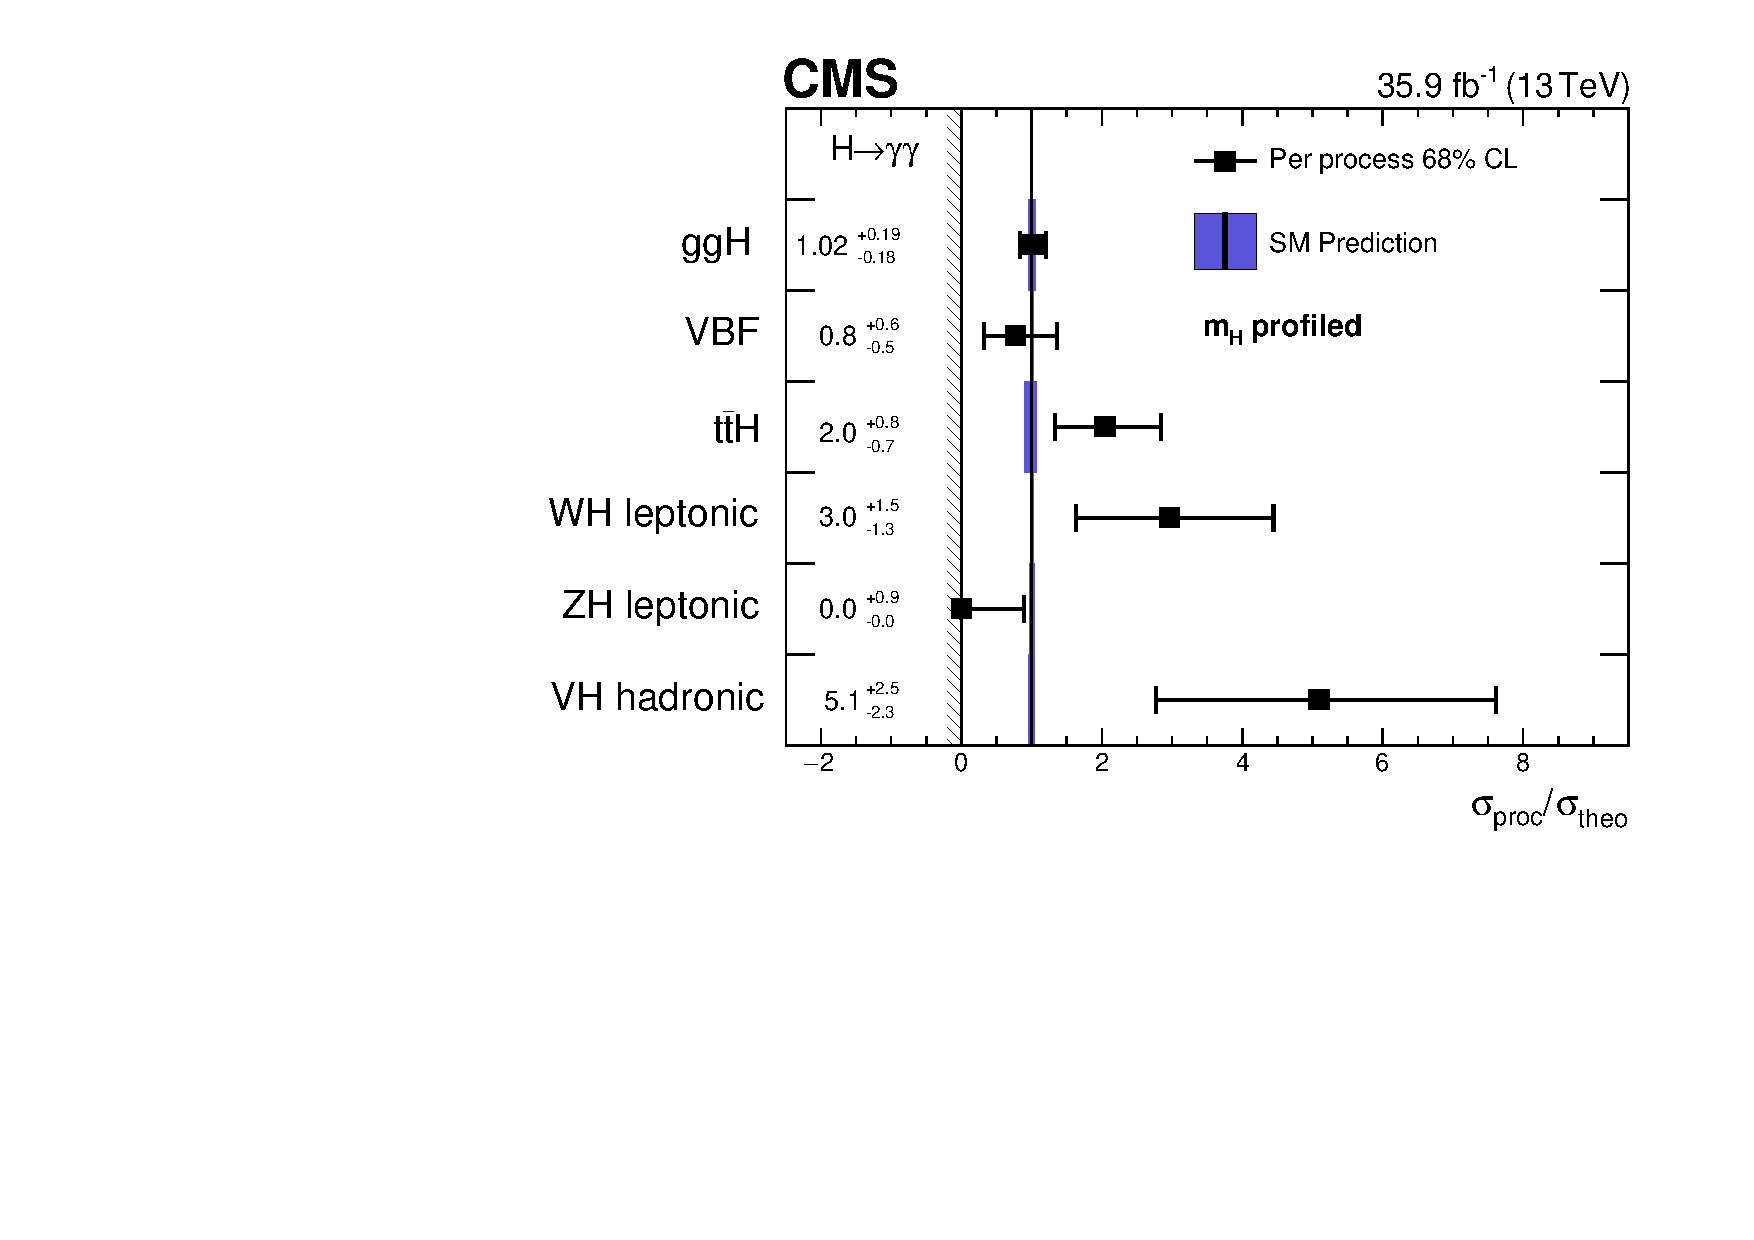
\includegraphics[width=0.75\textwidth]{figures/stats_results/CMS-HIG-16-040_Figure_018.pdf}
        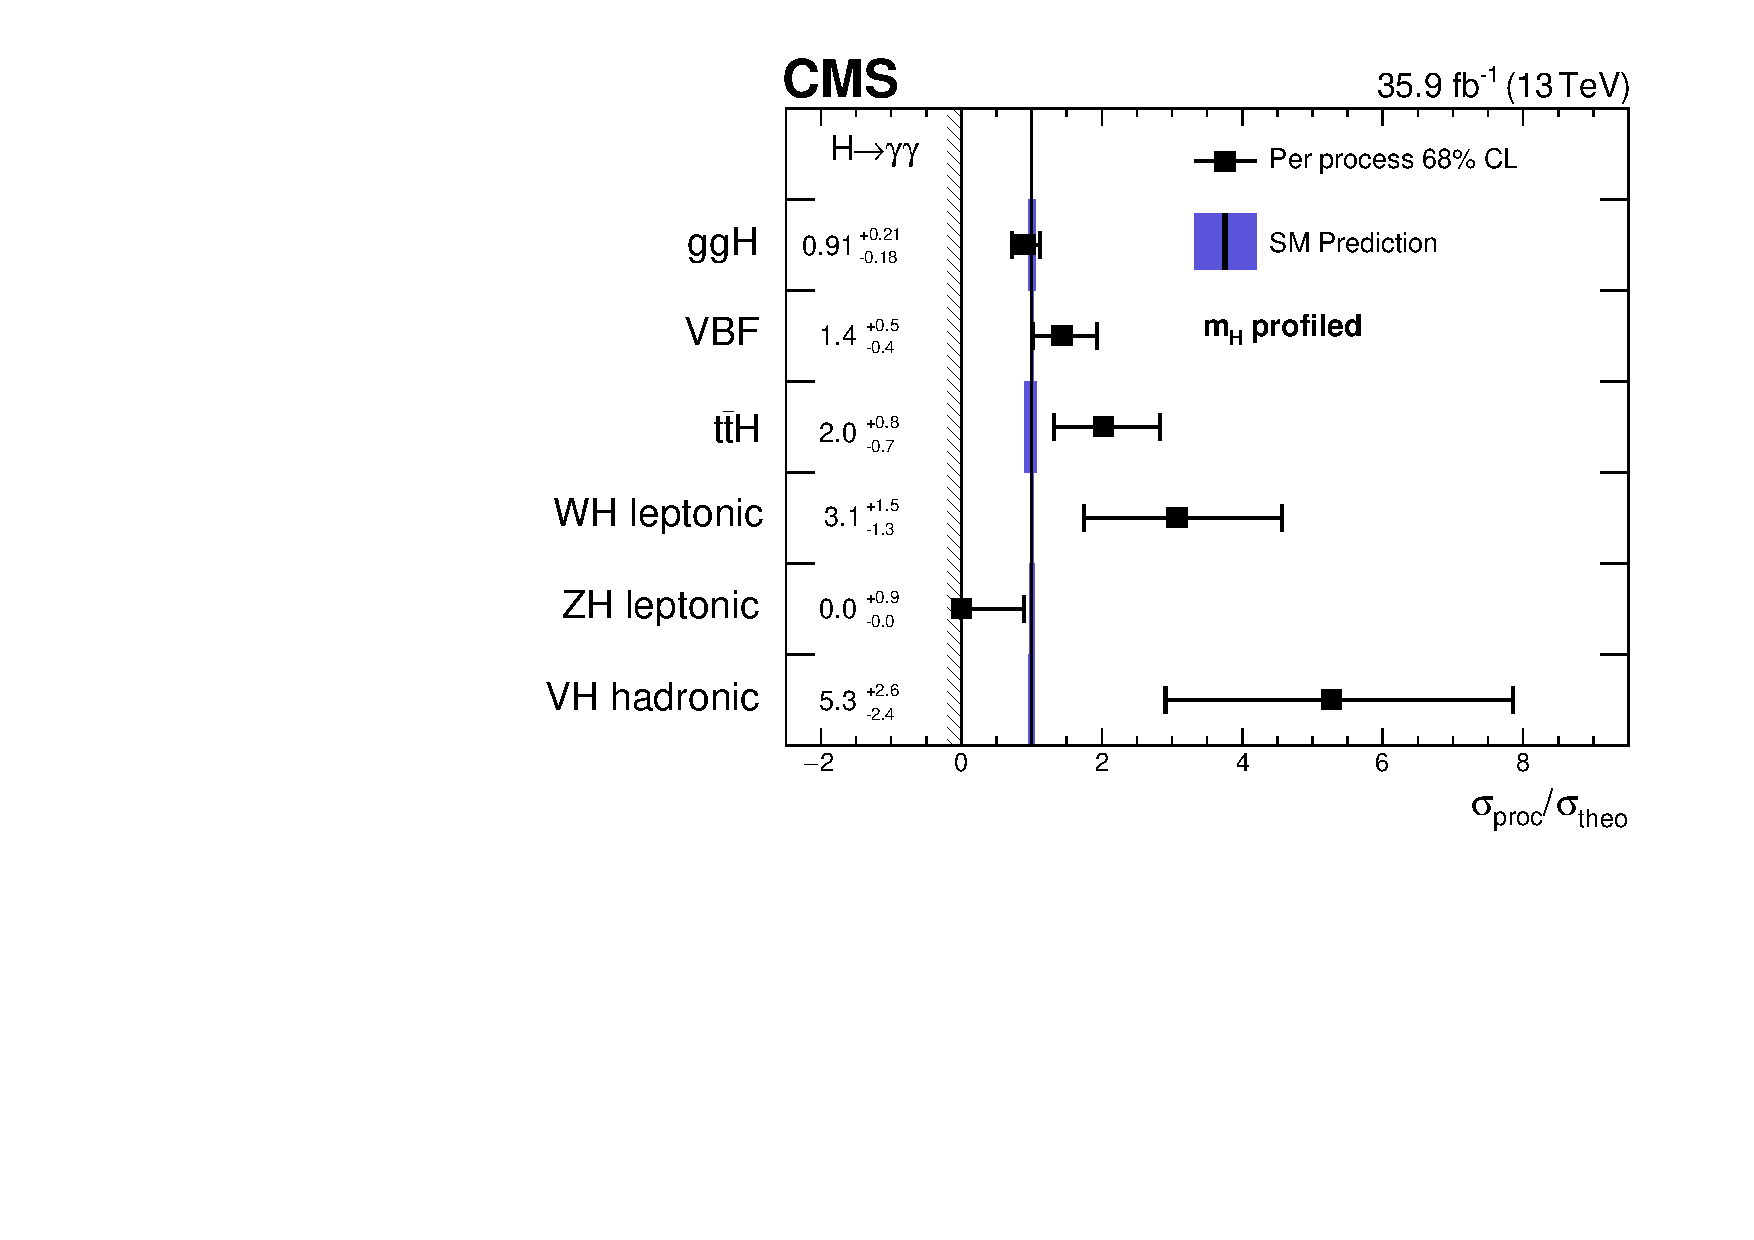
\includegraphics[width=0.75\textwidth]{figures/stats_results/STXSPerProcessMuProfileMH_ReMap.pdf}
    \end{center}
    \caption{SM prediction to measured cross section ratios in the STXS Stage 0 framework. Analysis with the BDT-based VBF tag is shown on top and the DCNN-based variant is on the bottom.}
        \label{fig:stats_results:stxs}
\end{figure}

The DCNN-based VBF tag has a similar effect in this scheme to the the production mode signal strengths. 






\subsubsection{Fermionic Versus Bosonic Production}
A measurement of the fermionic versus bosonic signal strength is performed with a 2D likelihood scan.
The procedure is similar to the above but with a signal strength for the bosonic production modes $\mu_{\mathrm{VBF},\mathrm{VH}}$ and the fermionic modes $\mu_{\mathrm{ggH},\mathrm{t\bar{t}H}}$.
A best fit point is found and then a $2\Delta\mathrm{NLL}$ test statistic is evaluated over a 2D space corresponding to different values of the two signal strength modifiers. 
The result with 68\% and 95\% confidence intervals is shown in Figure \ref{fig:stats_results:fermionic_bosonic}. 
\begin{figure}[h!]
    \begin{center}
        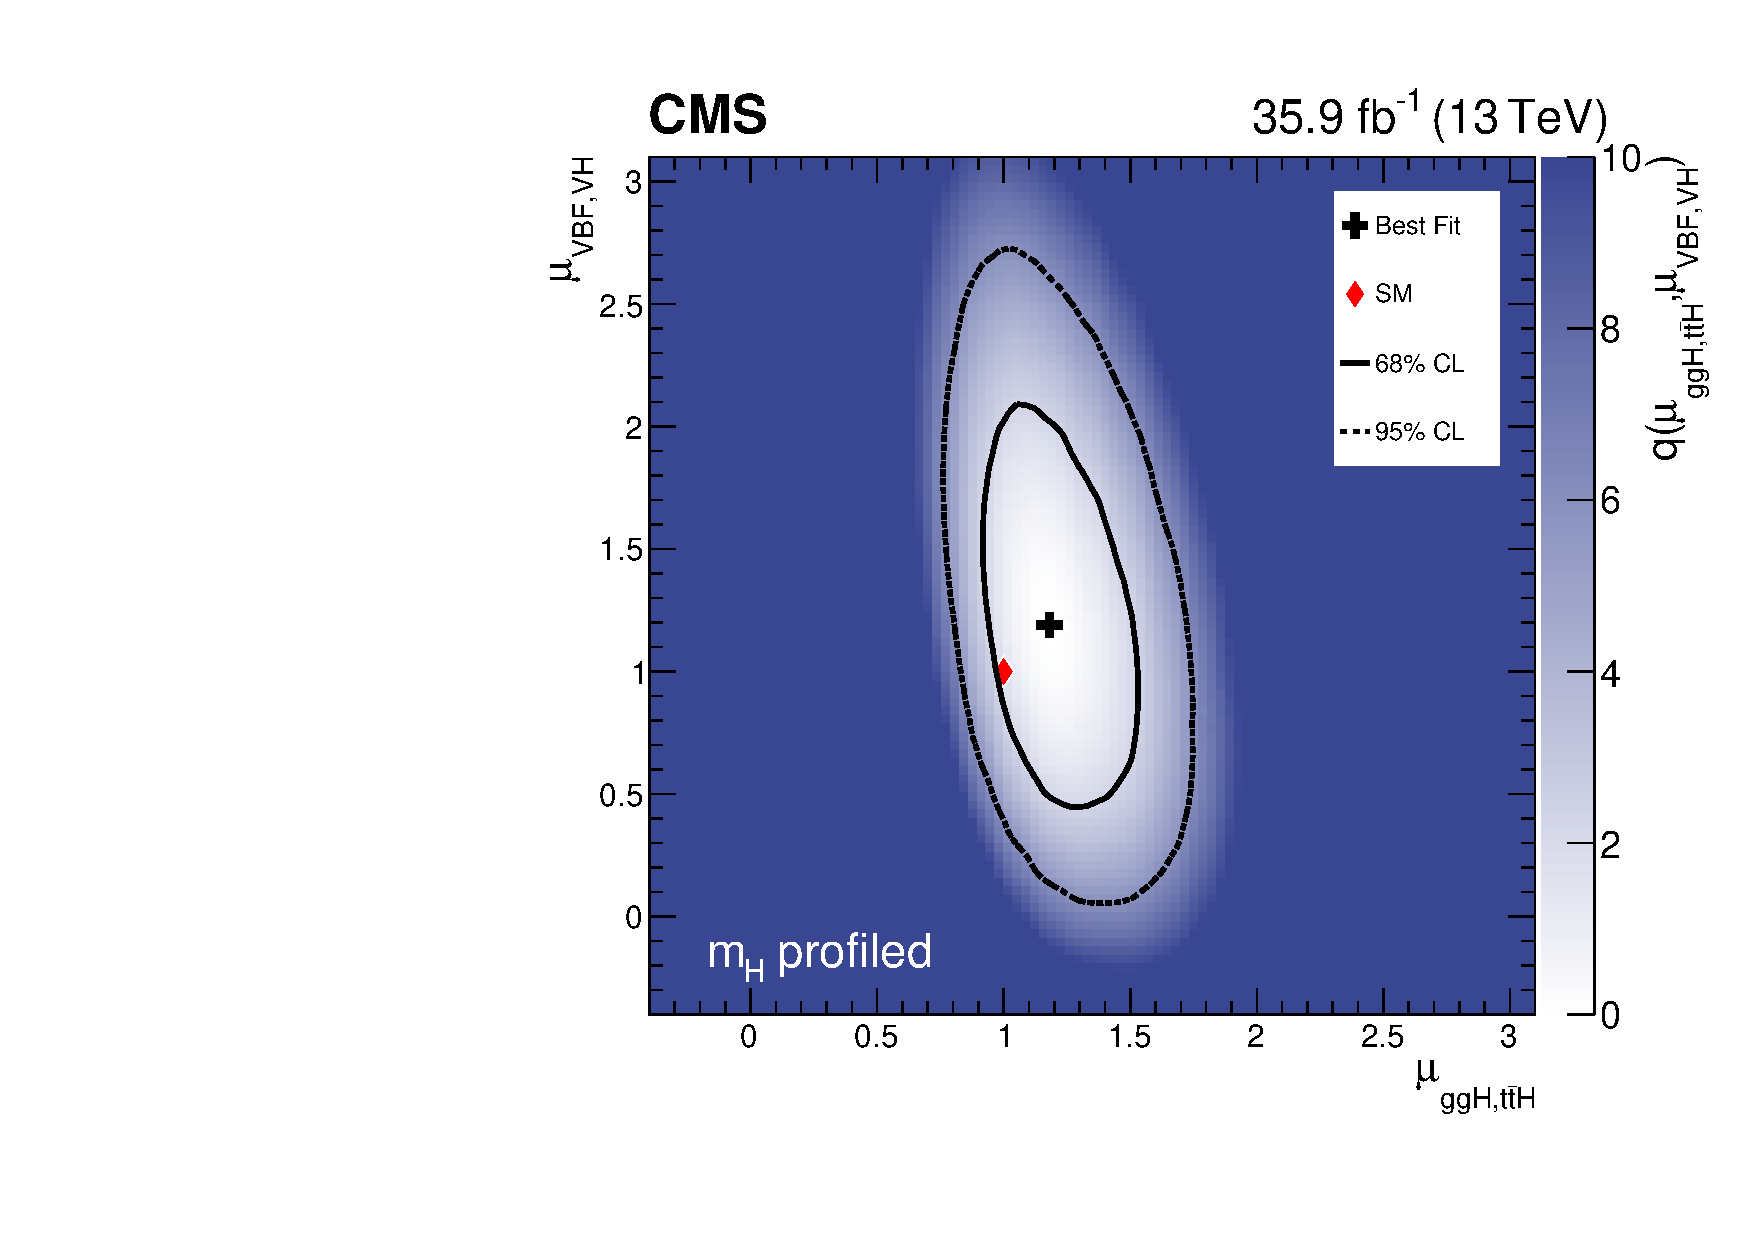
\includegraphics[width=0.49\textwidth]{figures/stats_results/CMS-HIG-16-040_Figure_019.pdf}
        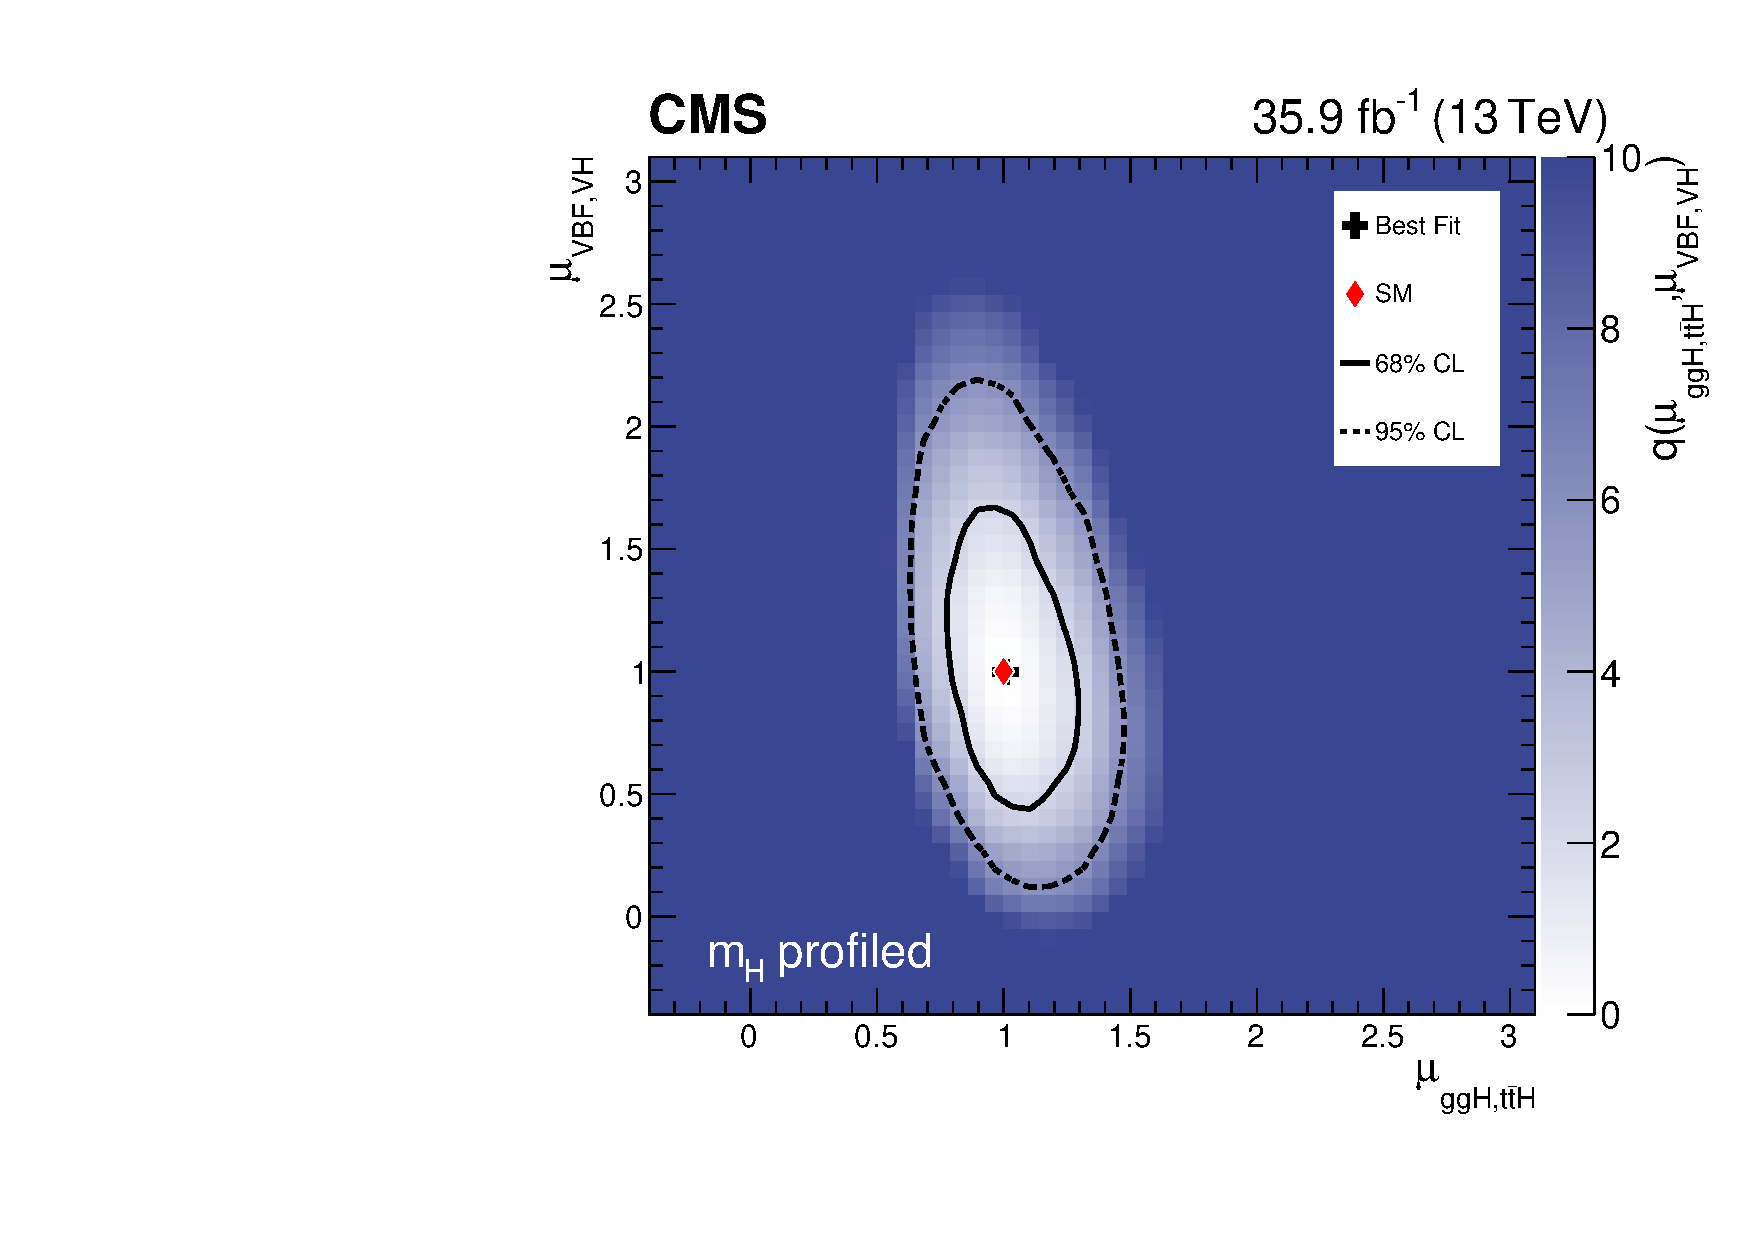
\includegraphics[width=0.49\textwidth]{figures/stats_results/RVRFScanProfileMH_col.pdf}
    \end{center}
    \caption{Two-dimensional likelihood scan of signal strength modifiers for bosonic (VBF, VH) and fermionic (ggH, \ttH) production modes. Analysis with the BDT-based VBF tag is shown on the left and the DCNN-based variant is on the right.}
        \label{fig:stats_results:fermionic_bosonic}
\end{figure}

The best fit point for the BDT-based case was found to be $\mu_{\mathrm{ggH},\mathrm{t\bar{t}H}} = 1.19^{+0.22}_{-0.18}$, $\mu_{\mathrm{VBF},\mathrm{VH}} = 1.21^{+0.58}_{-0.51}$.
The best fit point for the DCNN-based case was found to be $\mu_{\mathrm{ggH},\mathrm{t\bar{t}H}} = 1.11^{+0.20}_{-0.18}$, $\mu_{\mathrm{VBF},\mathrm{VH}} = 1.65^{+0.50}_{-0.42}$.
A significant reduction in the uncertainty of the bosonic production mode $\mu$ is observed along with an increase in its value.





\subsection{Couplings Measurements}
Deviation in the Higgs couplings from the SM expectation are modelled within the $\kappa$ framework as described in \cite{Kappa}.
These differences are measured with two 2D likelihood scans: fermionic versus bosonic and photons versus gluons.
The $\kappa$ values not subject to the 2D likelihood scan are fixed at unity.
The resulting plots for the BDT-based and DCNN-based VBF tags are shown in Figure \ref{fig:stats_results:kappa}.
\begin{figure}[h!]
    \begin{center}
        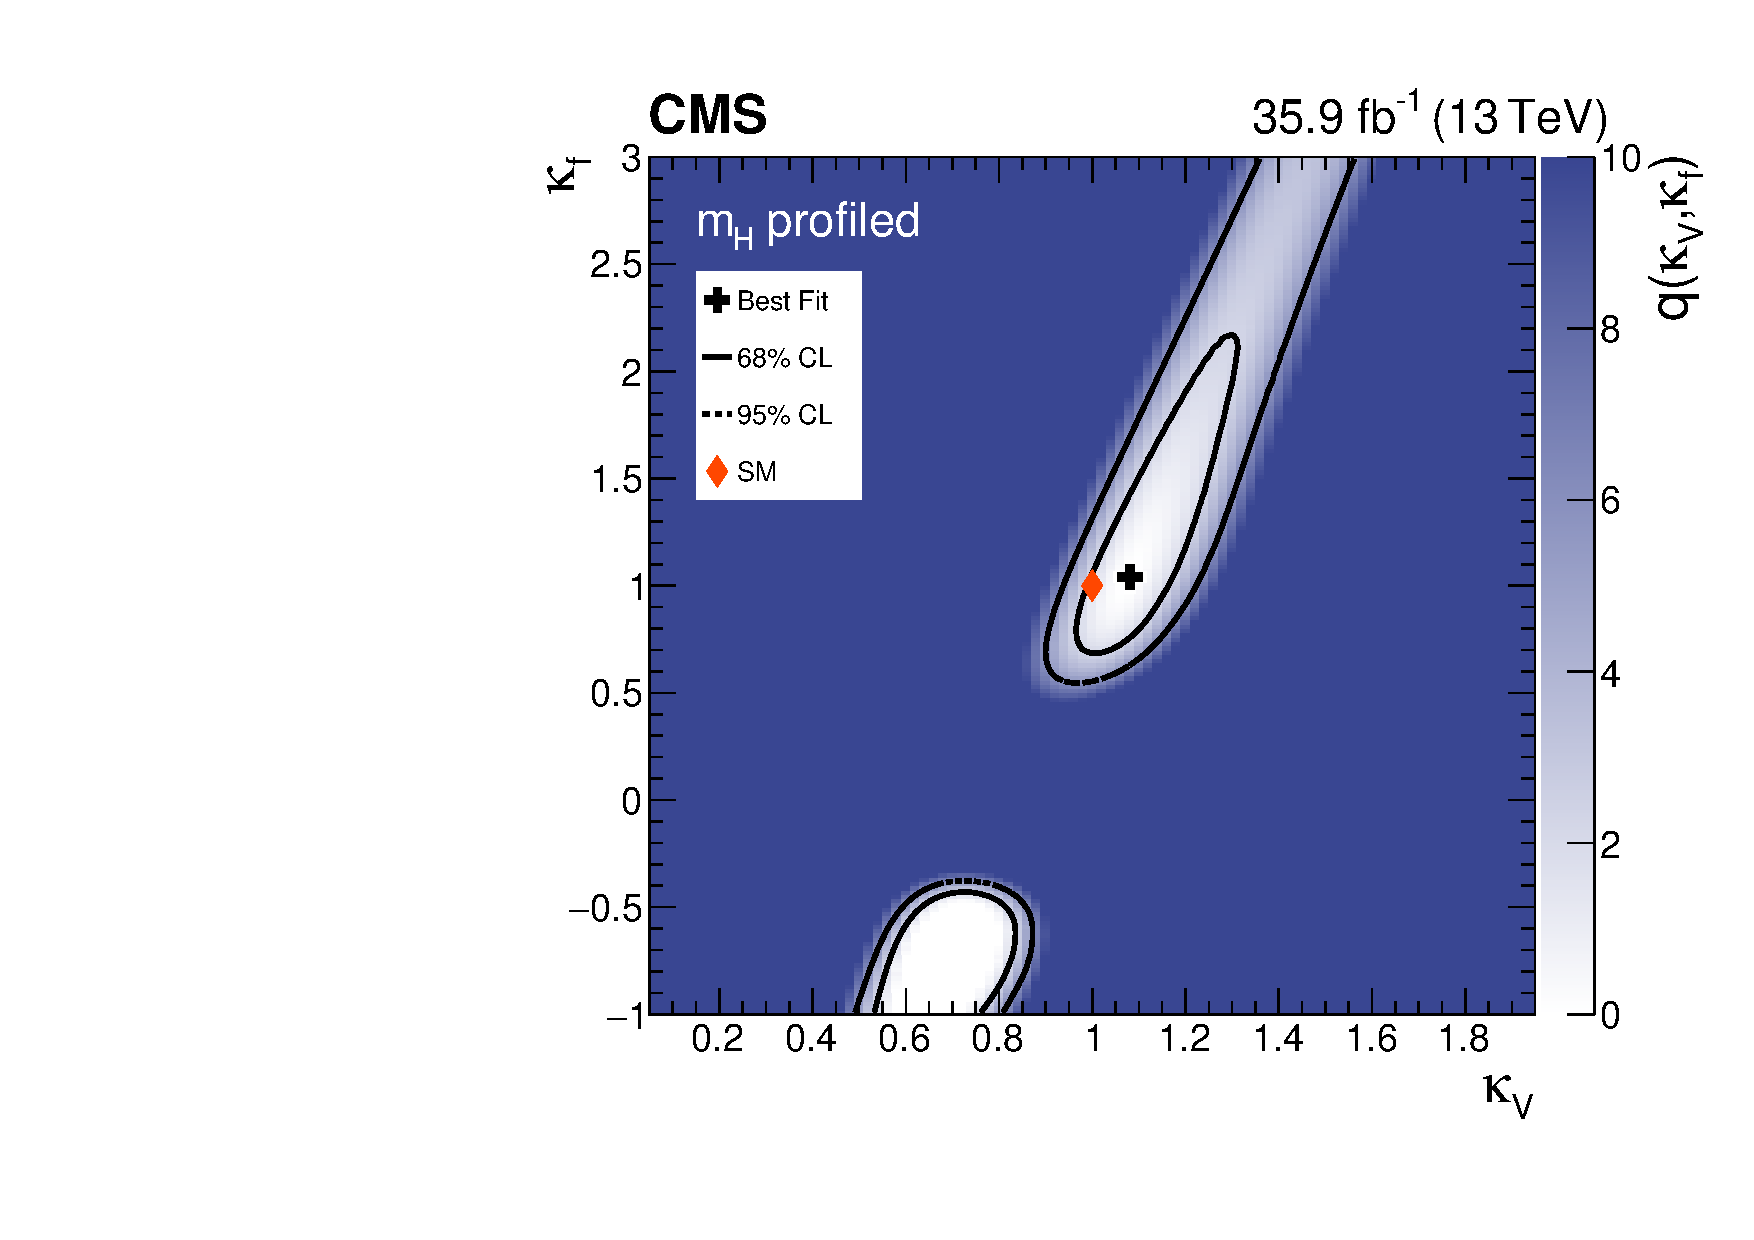
\includegraphics[width=0.49\textwidth]{figures/stats_results/CMS-HIG-16-040_Figure_020-a.pdf}
        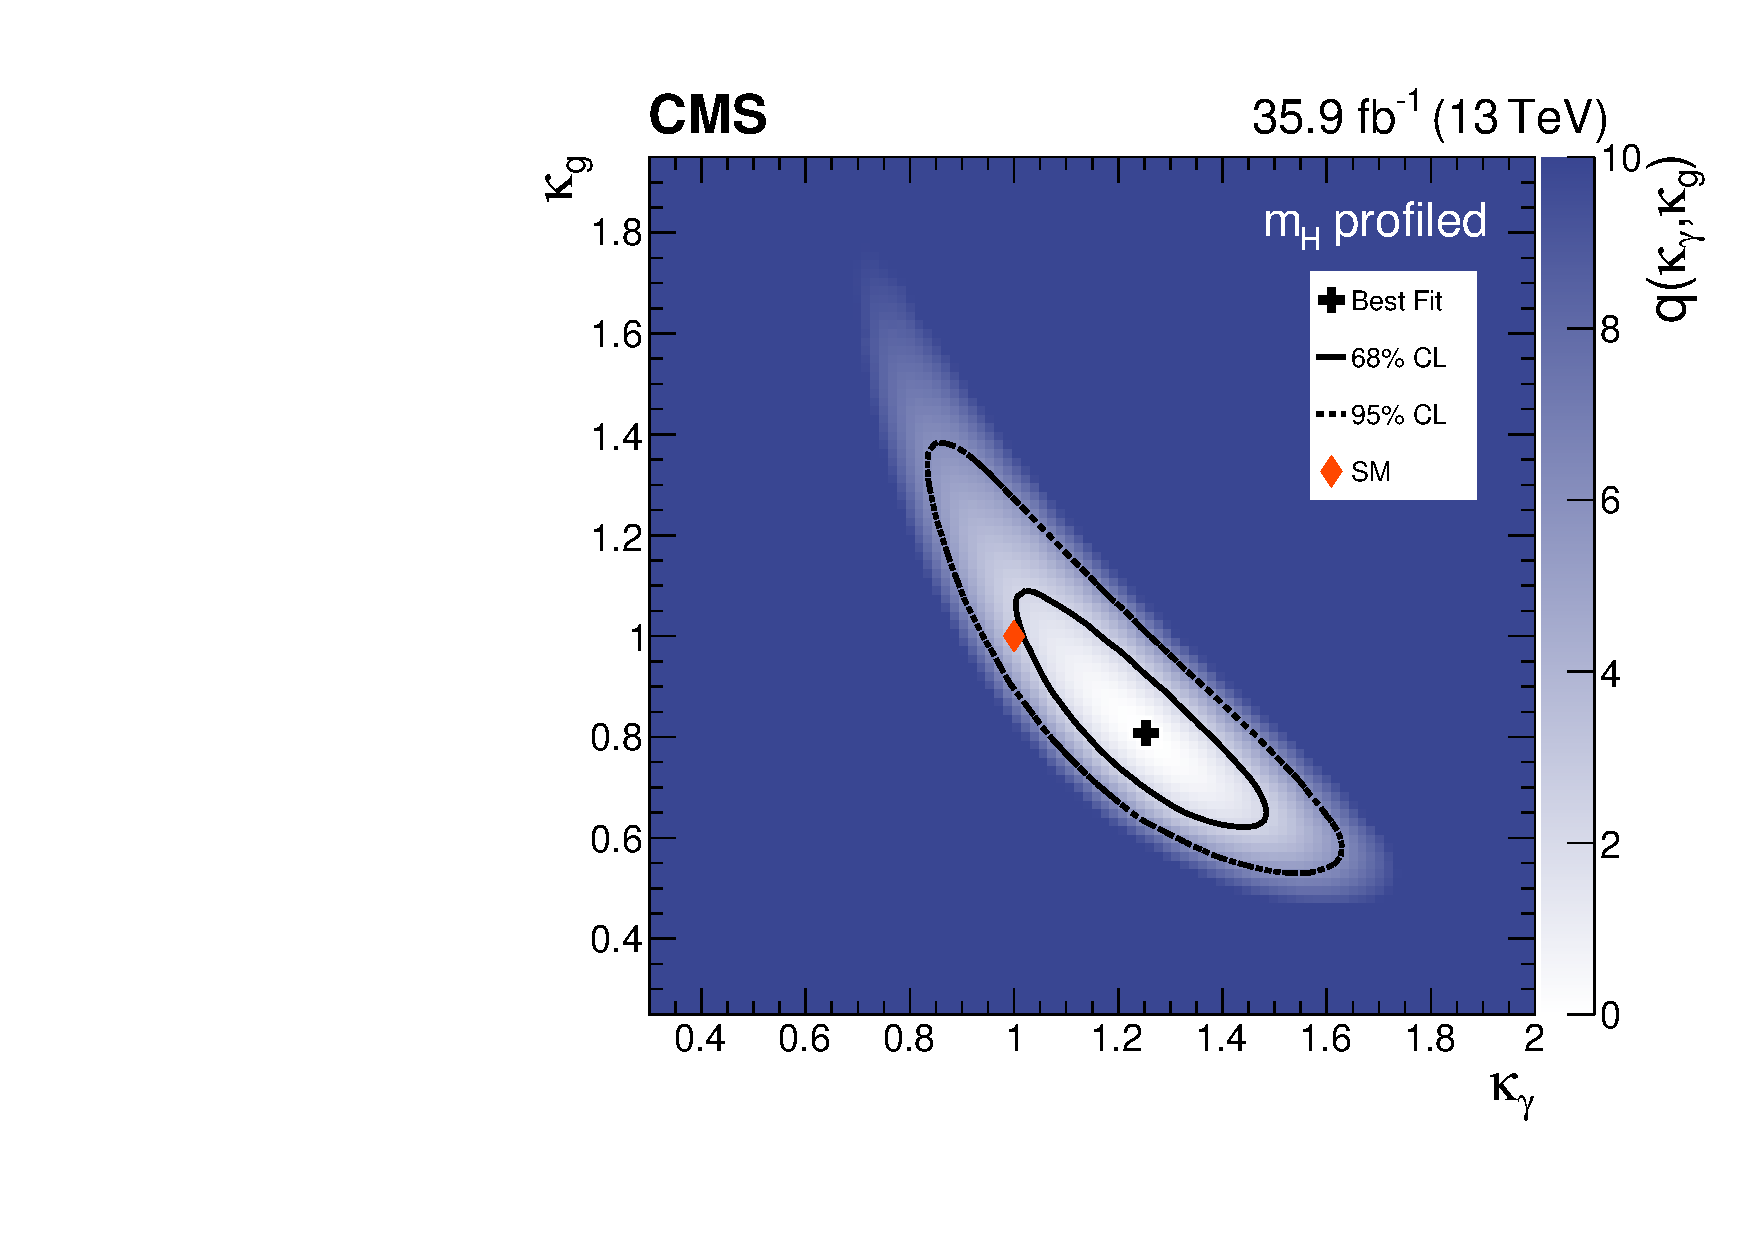
\includegraphics[width=0.49\textwidth]{figures/stats_results/CMS-HIG-16-040_Figure_020-b.pdf}
        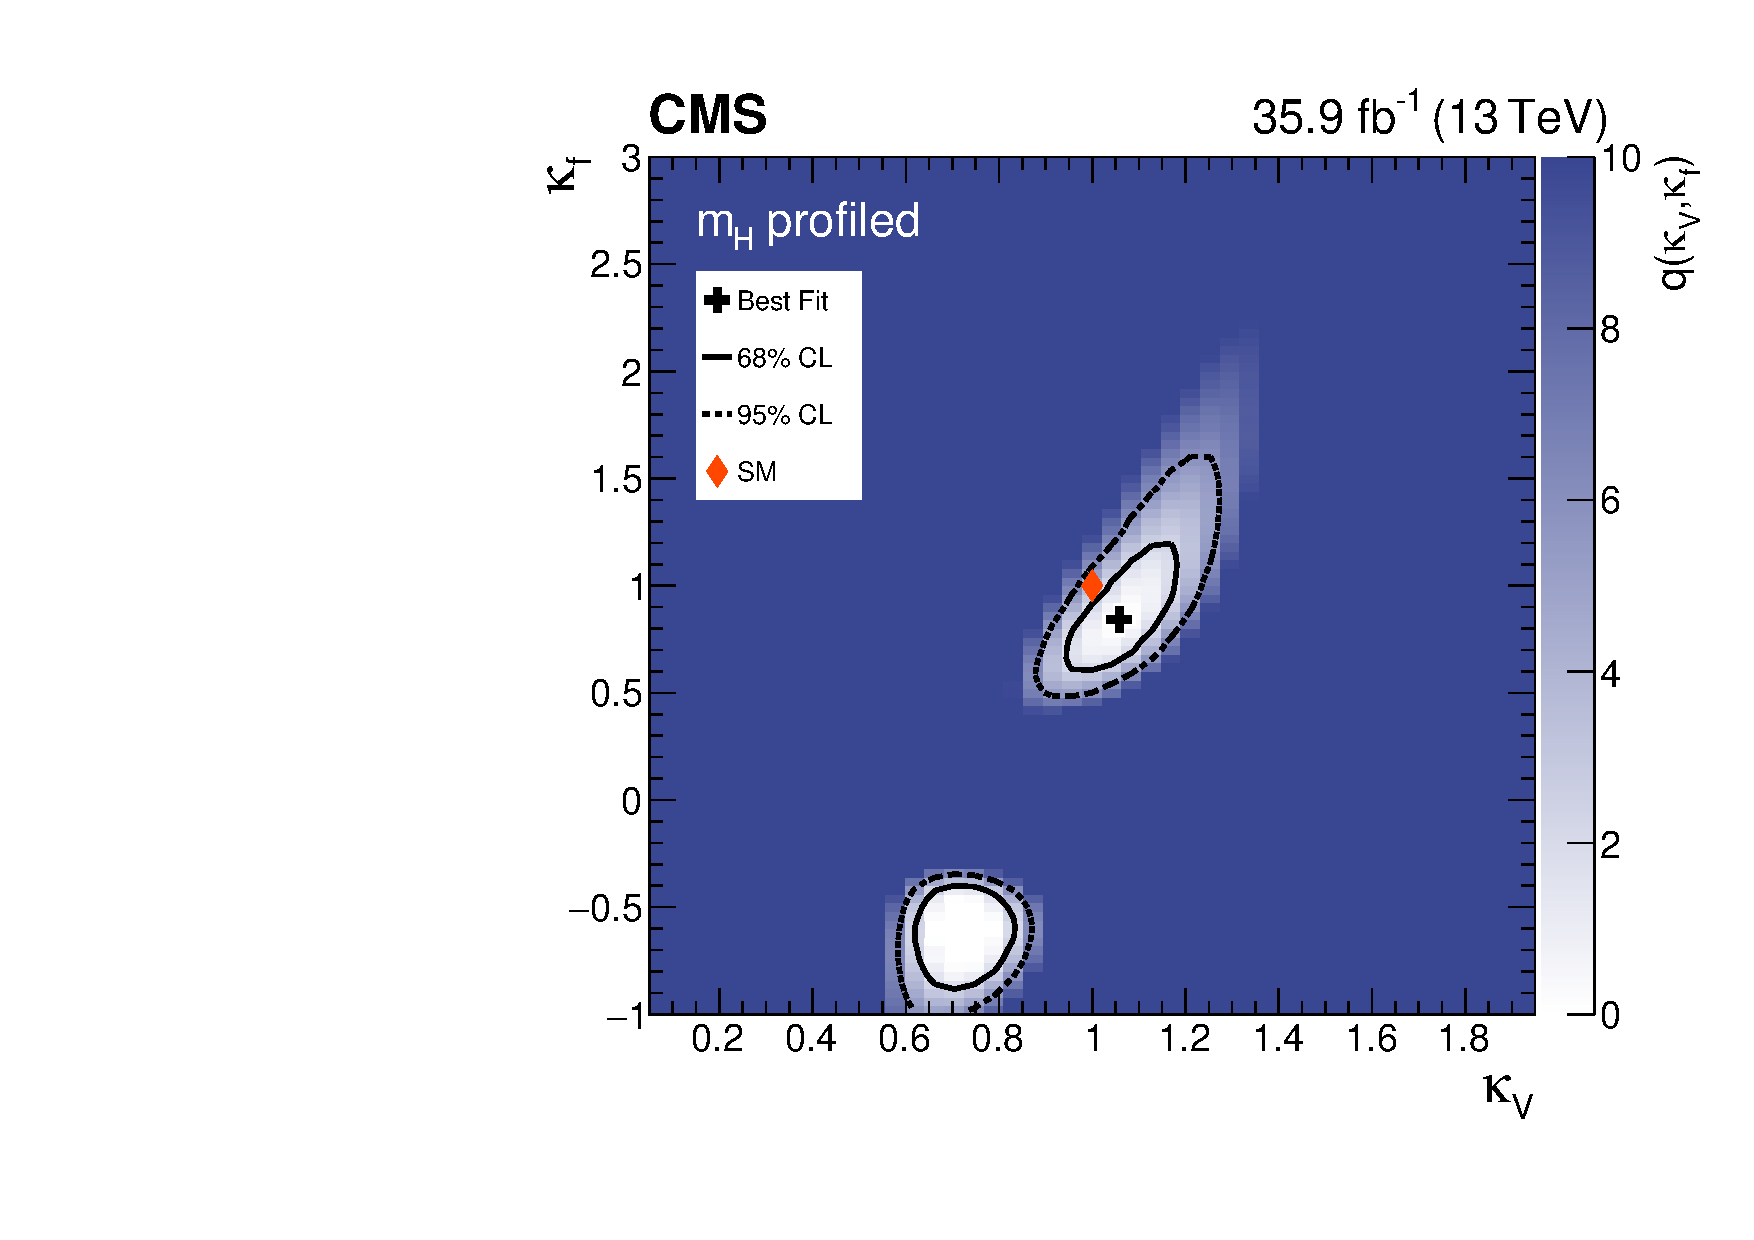
\includegraphics[width=0.49\textwidth]{figures/stats_results/CVCFScanProfileMH_col.pdf}
        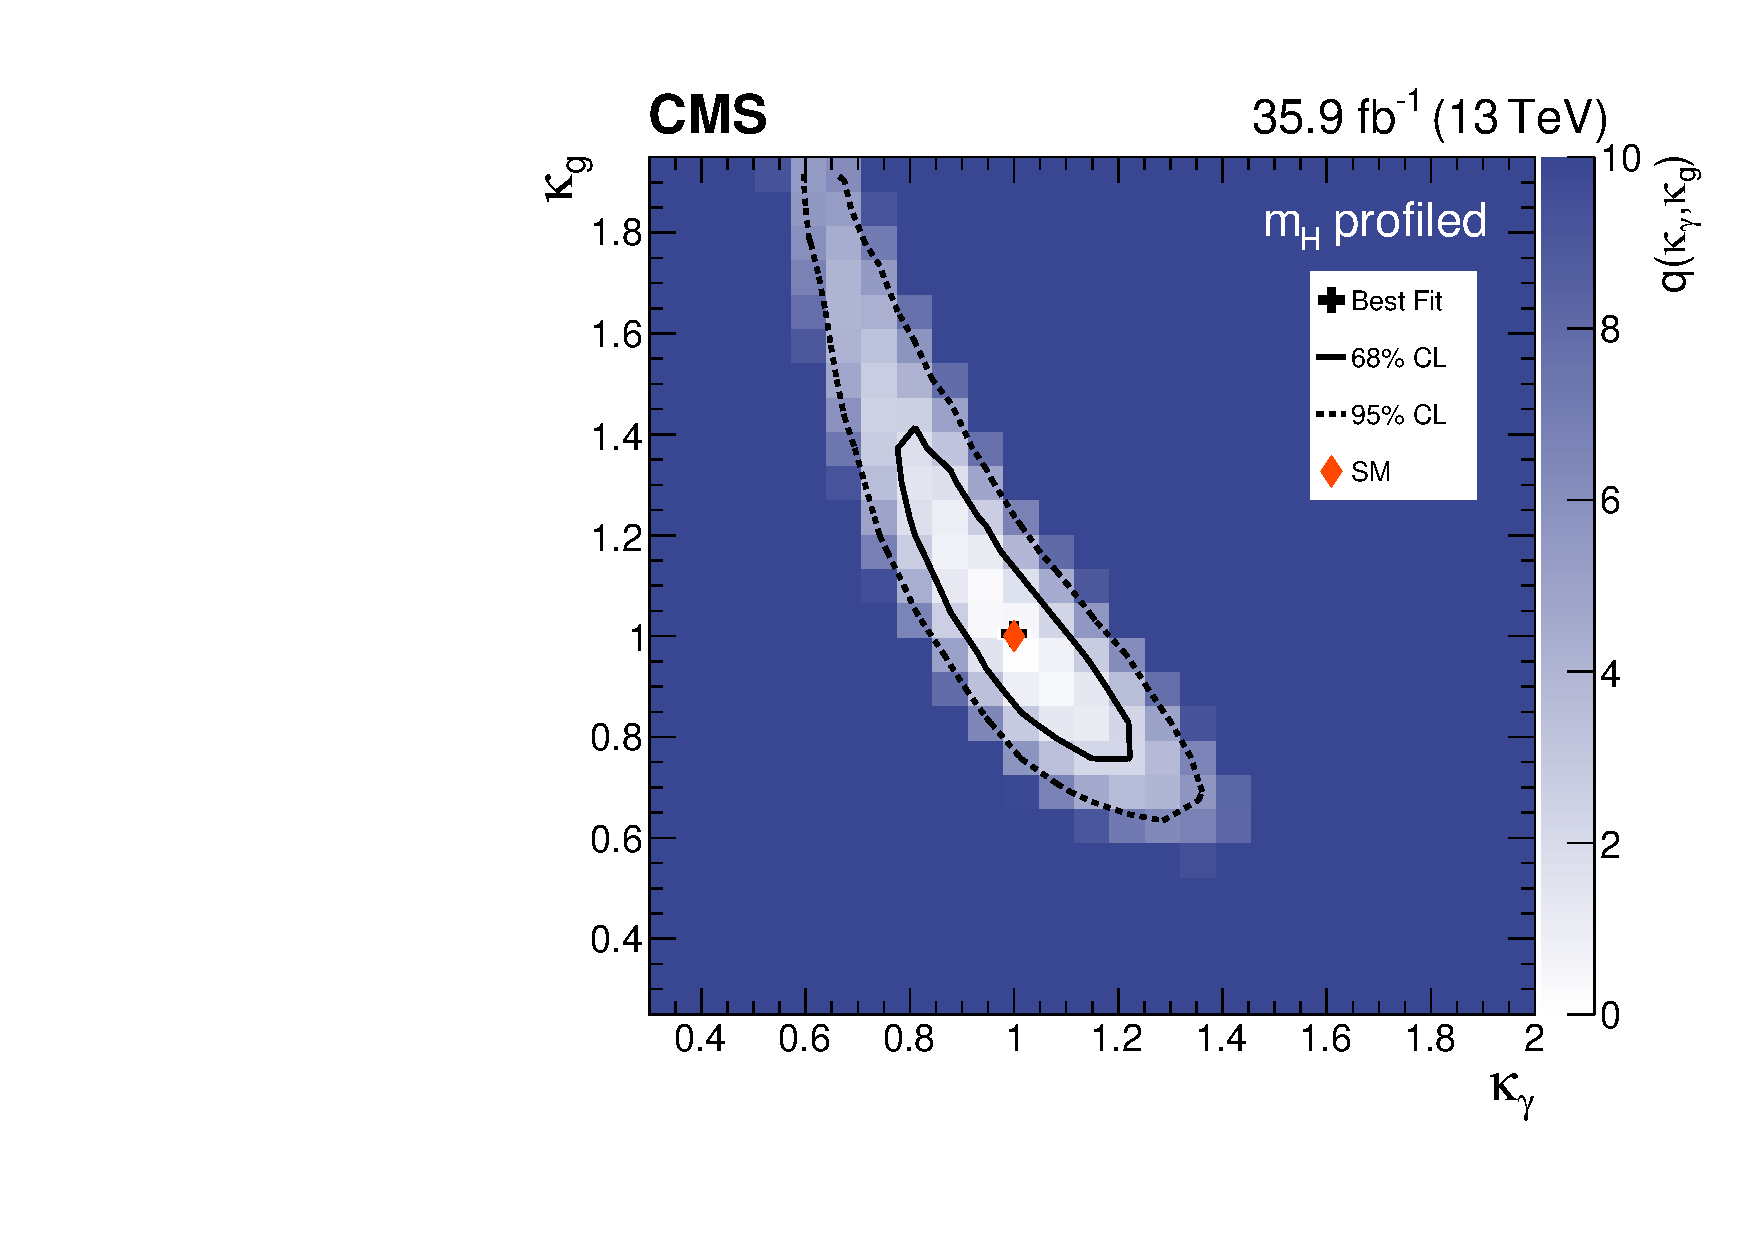
\includegraphics[width=0.49\textwidth]{figures/stats_results/KGluKGamScanProfileMH_col.pdf}
    \end{center}
    \caption{Two-dimensional likelihood scan of $\kappa$ values for bosonic versus fermionic production modes (left) and effective gluon coupling versus effective photon coupling (right).
             The BDT-based VBF tag is shown on the top, and the DCNN-based tag is shown at the bottom.}
        \label{fig:stats_results:kappa}
\end{figure}

With the BDT-based VBF tag the effective coupling to fermions is measured to be $\kappa_F=1.04^{+0.51}_{-0.25}$ and the effective coupling to bosons to be $\kappa_V=1.08^{+0.10}_{-0.08}$.
The effective coupling to photons is measured to be $\kappa_{\gamma}=1.25^{+0.16}_{-0.17}$ and the effective coupling to gluons to be $\kappa_{g}=0.81^{+0.17}_{-0.13}$.
With the DCNN-based VBF tag the effective coupling to fermions is measured to be $\kappa_F=0.85^{+0.22}_{-0.17}$ and the effective coupling to bosons to be $\kappa_V=1.06^{+0.07}_{-0.07}$.
The effective coupling to photons is measured to be $\kappa_{\gamma}=1.32^{+0.14}_{-0.13}$ and the effective coupling to gluons to be $\kappa_{g}=0.75^{+0.13}_{-0.13}$.


The DCNN-based case demonstrates a reduction in uncertainty in these measurements, especially for the couplings to bosons. 





\subsection{Conclusions}
A collection of measurements have been made comparing the BDT-based and DCNN-based VBF tags. 
The initial best fit to all categories shows an increase in expected signal purity and significance in the VBF production mode.
In the likelihood scans the DCNN is seen to bring improvement to some of the measurements. 
The greatest impact is seen in measurements of the VBF signal strength modifier itself, and on measurements of the bosonic signal strength and coupling modifiers.
All measurements are compatible with the SM.




